% !TeX spellcheck = en_GB
\documentclass{article}

\usepackage{fancyhdr}
\usepackage{titlesec}
\usepackage{titling}
\usepackage{extramarks}
\usepackage{lastpage}
\usepackage{libertine}
\usepackage{ifthen}
\usepackage[
	a4paper,
	total={135mm, 240mm},
	includehead,
	headsep=12mm,
	footskip=15mm
]{geometry}
\usepackage{amsmath}
\usepackage{amsthm}
\usepackage{amssymb}
\usepackage{mathtools}
\usepackage{graphicx}
\usepackage{color}
\usepackage[
	backend=biber,
	style=numeric,
	citestyle=authoryear,
	maxnames=10,
]{biblatex}
\usepackage{listings}
\usepackage{xparse}
\usepackage{multirow}
\usepackage{xcolor}
\usepackage{booktabs}
\usepackage{bookmark}
\usepackage{draftfigure}
\usepackage{bbm}
\usepackage{tabularx}
\usepackage{verbatim}
\usepackage[ruled, vlined]{algorithm2e}
\usepackage{doi}
\usepackage{hyperref}
\usepackage{placeins}
\usepackage{flafter}

\definecolor{blue}{HTML}{1f77b4}
\definecolor{orange}{HTML}{ff7f0e}
\definecolor{green}{HTML}{2ca02c}
\definecolor{red}{HTML}{d62728}
\definecolor{purple}{HTML}{9467bd}
\definecolor{brown}{HTML}{8c564b}

\addbibresource{mybib.bib}
\renewbibmacro{in:}{}

% Custom commands

\DeclarePairedDelimiter\abs{\lvert}{\rvert}
\DeclareMathOperator{\E}{E}
\DeclareMathOperator{\Var}{Var}
\newcommand{\R}{\mathbb{R}}
\newcommand{\Z}{\mathbb{Z}}
\newcommand{\N}{\mathbb{N}}
\newcommand{\dd}{{\rm d}}
\newcommand{\eps}{\varepsilon}

\newcommand{\st}{\textsuperscript{st}}
\newcommand{\nd}{\textsuperscript{nd}}
\newcommand{\rd}{\textsuperscript{rd}}
\renewcommand{\th}{\textsuperscript{th}}

\NewDocumentCommand{\codeword}{v}{%
	\texttt{\textcolor{blue}{#1}}%
}

\newtheorem{theorem}{Theorem}[section]
\newtheorem{lemma}[theorem]{Lemma}

\newcommand{\metro}[7]{
	\begin{tabularx}{\linewidth}{@{}Xl@{}}
		\toprule[0.1em]
		Proposal distributions &#1\\
		Initialisation &#2\\
		Sample size &#3\\
		\midrule[0.1em]
		\raisebox{-10mm}{Traceplots} &\raisebox{%
				3mm - \totalheight}{%
				\includegraphics[width=0.8\linewidth]{#4}}\\
		\raisebox{-8mm}{Histograms} &\raisebox{%
			3mm - \totalheight}{%
			\includegraphics[width=0.8\linewidth]{#5}}\\
		Acceptance rates &#6\\
		%Means&#7\\ 
		\bottomrule[0.1em]
	\end{tabularx}
}

\newcommand{\metroall}[3]{
	\begin{table*}
		\centering
		\renewcommand{\arraystretch}{1.2}
		\input{latex-bits/#1-G3-prior.txt}
		\caption{Metropolis-Hastings algorithm for
			$\pi_{\theta}^{\text{G3}}$ for #3}
		\label{table:#1-1}
	\end{table*}
	
	\begin{table*}
		\centering
		\renewcommand{\arraystretch}{1.2}
		\input{latex-bits/#1-G3-post.txt}
		\caption{Metropolis algorithm for
			$\pi^{\text{G3}}_{\theta \mid \mathbf{x}^{\text{#2}}}$ for #3}
	\end{table*}
	
	\begin{table*}
		\centering
		\renewcommand{\arraystretch}{1.2}
		\input{latex-bits/#1-G2-post.txt}
		\caption{Metropolis-Hastings algorithm for
			$\pi^{\text{G2}}_{\theta \mid \mathbf{x}^{\text{#2}}}$ for #3}
	\end{table*}
	
	\begin{table*}
		\centering
		\renewcommand{\arraystretch}{1.2}
		\input{latex-bits/#1-G1-post.txt}
		\caption{Metropolis-Hastings algorithm for
			$\pi^{\text{G1}}_{\theta \mid \mathbf{x}^{\text{#2}}}$ for #3}
	\end{table*}
	
	\begin{table*}
		\centering
		\renewcommand{\arraystretch}{1.2}
		\input{latex-bits/#1-MEC-prior.txt}
		\caption{Metropolis-Hastings algorithm for
			$\pi_{\theta}^{\text{MEC}}$ for #3}
	\end{table*}
	
	\begin{table*}
		\centering
		\renewcommand{\arraystretch}{1.2}
		\input{latex-bits/#1-MEC-post.txt}
		\caption{Metropolis-Hastings algorithm for
			$\pi^{\text{MEC}}_{\theta \mid \mathbf{x}^{\text{#2}}}$ for #3}
	\end{table*}

	\begin{table*}
		\centering
		\renewcommand{\arraystretch}{1.2}
		\input{latex-bits/#1-E-prior.txt}
		\caption{Metropolis-Hastings algorithm for
			$\pi_{\theta}^{\text{E}}$ for #3}
	\end{table*}
	
	\begin{table*}
		\centering
		\renewcommand{\arraystretch}{1.2}
		\input{latex-bits/#1-E-post.txt}
		\caption{Metropolis-Hastings algorithm for
			$\pi^{\text{E}}_{\theta \mid \mathbf{x}^{\text{#2}}}$ for #3}
	\end{table*}

	\begin{table*}
		\centering
		\renewcommand{\arraystretch}{1.2}
		\input{latex-bits/#1-TN-prior.txt}
		\caption{Metropolis-Hastings algorithm for
			$\pi_{\theta}^{\text{TN}}$ for #3}
	\end{table*}
	
	\begin{table*}
		\centering
		\renewcommand{\arraystretch}{1.2}
		\input{latex-bits/#1-TN-post.txt}
		\caption{Metropolis-Hastings algorithm for
			$\pi^{\text{TN}}_{\theta \mid \mathbf{x}^{\text{#2}}}$ for #3}
		\label{table:#1-2}
	\end{table*}
}

\newcommand{\marginals}[7]{
	\begin{table*}
		\centering
		\renewcommand{\arraystretch}{1.2}
		\begin{tabular}{@{}cc@{}}
			\toprule[0.1em]
			\raisebox{%
					-\totalheight}{%
					\includegraphics[%
						width=0.97\linewidth]{%
						plots/#1-#3-#6-0-marg.pdf}} \\
			\midrule[0.1em]
			\raisebox{%
					-\totalheight}{%
					\includegraphics[%
						width=0.97\linewidth]{%
						plots/#1-#3-#6-1-marg.pdf}} \\
			\midrule[0.1em]
			\raisebox{%
					-\totalheight}{%
					\includegraphics[%
						width=0.97\linewidth]{%
						plots/#1-#3-#6-2-marg.pdf}} \\
			\bottomrule[0.1em]
		\end{tabular}
		\caption{Prior and posterior #5 marginals of #4
			for #2#7}
		\label{table:#1-#3-#6-marg}
	\end{table*}
}

\newcommand{\allmarginals}[2]{
	\marginals{#1}{#2}{theta}{$\theta$}{univariate}{0}{%
		, with dashed lines for improper priors}
	\marginals{#1}{#2}{theta}{$\theta$}{bivariate}{1}{%
		, with dashed lines for improper priors}
	\marginals{#1}{#2}{q}{$(q_1, q_2, q_3)$}{univariate}{0}{}
	\marginals{#1}{#2}{q}{$(q_1, q_2, q_3)$}{bivariate}{1}{%
		, with grey shaded region $x < y$}
}

\newcommand{\allreturnlevels}[2]{
	\begin{table*}
		\centering
		\renewcommand{\arraystretch}{1.2}
		\begin{tabular}{@{}ccc@{}}
			\raisebox{-\totalheight}{%
				\includegraphics[%
					width=0.46\linewidth]{%
					plots/#1-G3-post-return-level.pdf}}
				&\raisebox{%
					-\totalheight}{%
					\includegraphics[%
						width=0.46\linewidth]{%
						plots/#1-MEC-post-return-level.pdf}} \\
			\raisebox{-\totalheight}{%
				\includegraphics[%
					width=0.46\linewidth]{%
					plots/#1-G2-post-return-level.pdf}}
				&\raisebox{%
					-\totalheight}{%
					\includegraphics[%
						width=0.46\linewidth]{%
						plots/#1-G1-post-return-level.pdf}} \\
			\raisebox{-\totalheight}{%
				\includegraphics[%
					width=0.46\linewidth]{%
					plots/#1-E-post-return-level.pdf}}
				&\raisebox{%
					-\totalheight}{%
					\includegraphics[%
						width=0.46\linewidth]{%
						plots/#1-TN-post-return-level.pdf}} \\
		\end{tabular}
		\caption{Mean return level with 95\% credibility intervals
			estimated using various posterior distributions,
			with analytic return level {\color{black} \textbf{(black solid)}},
			simulated return level {\color{black} \textbf{(black dashed)}}
			and empirical quantiles {\color{black} \textbf{(black dots)}}
			for #2}
		\label{table:#1-post-return-level}
	\end{table*}
}

%%% Style

\newcommand{\hwtitle}{Report version 11}
\newcommand{\hwdate}{1\st July 2020}
\newcommand{\hwname}{Tony Zheng}

\title{%
	\vspace{-15mm}\Huge{\hwtitle}\\
	\Large\vspace{1mm}\hwname\\
	\Large\vspace{1mm}\small{\itshape\hwdate}\vspace{-15mm}}
\date{}
\author{}

\pagestyle{fancy}
\lhead{\hwname}
\chead{\hwtitle}
\rhead{\firstxmark}
\lfoot{\lastxmark}
\cfoot{}
\rfoot{Page\ \thepage\ of\ \pageref{LastPage}}
\renewcommand\headrulewidth{0.4pt}
\renewcommand\footrulewidth{0.4pt}

\fancypagestyle{plain}{%
	\renewcommand{\headrulewidth}{0pt}%
	\fancyhf{}%
	\lfoot{\lastxmark}
	\cfoot{}
	\rfoot{Page\ \thepage\ of\ \pageref{LastPage}}
}

\allowdisplaybreaks

\begin{document}
%	
\maketitle
%
\section{Introduction}
%

%
The study of environmental conditions is crucial
in the development of large scale construction projects.
In particular, the study of long-term behaviour
of environmental variables is necessary to understand
the risks of hazardous meteorological events such as
floods, storms, and droughts.
This can be done using the well-established theory of extreme values,
using asymptotic models such as the Process point process characterisation
of extremes described in \cite{coles2001}.
However, the analysis of extreme events is often hindered
by a scarcity of data, and an inadequate treatment
of model and prediction uncertainties.
To overcome these problems, a Bayesian methodology has been proposed.
This approach allows us to exploit prior information,
and provides a framework for taking into account the various uncertainties
in the prediction process.
%

%
A review of the use of Bayesian methods in extreme value theory
has been carried out in \cite{coles1996review},
and analyses have been performed in both \cite{coles2003} and \cite{coles1996}
to predict annual maximum rainfall.
In the latter, Coles and Tawn employ the Poisson point process model,
and elicit prior information specified by an expert in the domain.
In this paper, we will attempt to replicate the analysis of \cite{coles1996}
using alternative prior distributions.
We will construct these distributions with the principle
of maximum entropy in mind, which results in more uninformative priors.
This will account for uncertainty due to lack of information in the model.
In particular, we will propose a novel technique in prior elicitation
in which a maximum entropy joint distribution
is constructed from given marginals.
%

%
In \S~\ref{section:distributions}, we will define the distributions
which we will use throughout the report.
In \S~\ref{section:model}, we will outline the Poisson point process model.
In \S~\ref{section:priors}, we will describe the original prior distribution
used by \cite{coles1996}, and propose alternative prior distributions.
In \S~\ref{section:mcmc}, we will explain how Markov chain Monte Carlo (MCMC)
methods can be used in the analysis to avoid intractable calculations.
In \S~\ref{section:studies}, we will implement and compare our priors
in simulation studies and on real wind speed data.
Finally, in the Appendix we have supplementary calculations
and details of our MCMC implementations.
%
\section{Named distributions}
\label{section:distributions}
%

%
\subsection{Generalised extreme value distribution}
%

%
The generalised extreme value (GEV) has CDF
%
\begin{align}
	F(x) =
		\begin{cases}
			\exp\left(-\left\{1 + \xi
			\left(\frac{x - \mu}{\sigma}\right)\right\}_+
			^ {-\frac{1}{\xi}}\right)
			&\quad \text{if $\xi \neq 0$} \,,\\
			\exp(-\exp(-\frac{x - \mu}{\sigma}))
			&\quad \text{if $\xi = 0$} \,,
		\end{cases}
	\label{eq:GEV-CDF}
\end{align}
%
where $\{x\}_+ \coloneqq \max\{0, x\}$, with parameters
$\theta \coloneqq (\mu, \sigma, \xi)$ defined in the set
%
\begin{align}
	\Theta \coloneqq \R \times \R^+ \times \R \,.
	\label{eq:Theta}
\end{align}
%
\subsection{Gamma distribution}
%

%
A random variable $X$ follows a Gamma distribution
with shape $\alpha \in \R^+$ and rate $\beta \in \R^+$
if it has PDF
%
\begin{align*}
	f(x) = \frac{\beta ^ \alpha x ^ {\alpha - 1} \exp(-\beta x)}{\Gamma(\alpha)}
	\mathbbm{1}_{x > 0} \,,
\end{align*}
%
where $\Gamma$ is the gamma function.
This is denoted $X \sim \Gamma(\alpha, \beta)$.
%
\subsection{Truncated normal distribution}
%

%
Suppose that $Y$ is a random variable which follows a normal distribution
with mean $\mu \in \R$ and variance $\sigma \in \R^+$.
For $\infty \leq a < b \leq \infty$,
the random variable $X \coloneqq Y \mid Y \in (a, b)$
follows a truncated normal distribution with PDF
%
\begin{align*}
	f(x) &= \frac{1}{\sigma} \frac{\phi(\frac{x - \mu}{\sigma})}
		{\Phi(\frac{b - \mu}{\sigma}) - \Phi(\frac{a - \mu}{\sigma})}
		\mathbbm{1}_{a < x < b} \,,
\end{align*}
%
where $\phi$ and $\Phi$ are the PDF and CDF of the
standard normal distribution respectively.
This is denoted $X \sim \operatorname{TN}(\mu, \sigma, a, b)$.
The parameters are $\mu$ and $\sigma$, the parent mean and standard deviation respectively, and the (possibly infinite) bounds $a$ and $b$.
%
\subsection{Exponential distribution}
%

%
A random variable $X$ follows an exponential distribution
with rate $\lambda \in \R^+$ if it has PDF
%
\begin{align*}
	f(x) = \lambda \exp(-\lambda x) \mathbbm{1}_{x > 0}
\end{align*}
%
This is denoted $X \sim \operatorname{Exp}(\lambda)$.
%
\section{Likelihood model}
\label{section:model}
%

%
Extreme values are often modelled using the GEV distribution.
Given a sequence of i.i.d. variables $X_1, \dots, X_n$,
under certain conditions,
its maximum
\begin{align*}
	M_n \coloneqq \max\{X_1, \dots, X_{n}\}
\end{align*}
asymptotically follows a GEV distribution as $n \to +\infty$.
%

%
The Poisson point process characterisation of extremes~(\cite{coles2001})
is an alternative model which takes into account
all extreme observations in the data,
i.e. all observations which are greater than some threshold $u$.
We will ignore the asymptotic nature of the model.
Suppose that we have daily observations of $X$ over $M$ years.
Denote by $\mathbf{x}=(x_1, \dots, x_{n_u})$
the exceedances of our data by some threshold $u$.
The likelihood of the data is then a non-homogeneous
Poisson point process
%
\begin{align}
	L(\theta \mid \mathbf{x})
		= \exp \left(-M \Lambda[u, \infty)\right)
		\prod_{i = 1}^{n_u} \lambda(x_i) \,,
	\label{eq:likelihood}
\end{align}
%
with intensity function
%
\begin{align}
	\lambda(x) \coloneqq
	\begin{cases}
		\frac{1}{\sigma}
			\left\{1 + \xi \left(\frac{x - \mu}{\sigma}\right)\right\}_+
			^ {-\frac{\xi + 1}{\xi}}
			&\quad \text{if $\xi \neq 0$} \,,\\
		\frac{1}{\sigma}\exp(-\frac{x - \mu}{\sigma})
			&\quad \text{if $\xi = 0$} \,,
	\end{cases}
	\label{eq:GP}
\end{align}
%
and
% 
\begin{align}
	\Lambda[u, \infty) &\coloneqq \int_u ^ \infty \lambda(x) \, \dd x \\
	&=
		\begin{cases}
			\left\{1 + \xi \left(\frac{u - \mu}{\sigma}\right)\right\}_+
			^ {-\frac{1}{\xi}}
			&\quad \text{if $\xi \neq 0$} \,,\\
			\exp(-\frac{u - \mu}{\sigma})
			&\quad \text{if $\xi = 0$} \,.
		\end{cases}
	\label{eq:Lambda}
\end{align}
%
This is an extension of the GEV model,
as the annual maxima $M_{365}$
follow a GEV distribution with parameters $\theta$.
%

%
Inverting \eqref{eq:GEV-CDF}, we obtain the quantile function
%
\begin{align}
	q(p \mid \mu, \sigma, \xi) &=
	\begin{cases}
		\mu + \frac{\sigma}{\xi} (\exp(-\log(-\log(p)) \xi) - 1)
			&\quad \text{if $\xi \neq 0$}\,,\\
		\mu - \sigma \log(-\log(p))
			&\quad \text{if $\xi = 0$} \,.
	\end{cases}
	\label{eq:quantile}
\end{align}
%
Of particular interest to us are the quantiles
corresponding to very small probabilities.
The \textit{return level} of a \textit{return period} $r$ in years
is defined as the quantile $q(1 - 1 / r\mid \theta)$.
%
\section{Eliciting prior information}
\label{section:priors}
%
Bayesian inference is centred around the use of Bayes' theorem
to update prior belief when new data is observed.
This prior belief is incorporated
into the model in the form of a prior distribution for the parameters.
In our case, we assume that this information
arises from the opinion of an expert.
Unfortunately, it is not feasible to specify joint distributions
for the parameters $\theta$.
Instead, we will consider prior distributions
for quantiles of the annual maxima.
%

%
Let $1 > p_1 > p_2 > p_3 > 0$ be a decreasing sequence of probabilities,
and for $i = 1, 2, 3$, consider the corresponding $(1 - p_i)$-quantiles
%
\begin{align}
	q_i &\coloneqq q(1 - p_i \mid \theta) \,, \nonumber \\
	&= \mu + \frac{\sigma}{\xi} (\exp(s_i \xi) - 1) \,,
	\label{eq:q_i}
\end{align}
%
where $q$ is defined in \eqref{eq:quantile}
and $s_i \coloneqq -\log(-\log(1 - p_i))$.
We are assuming that $\xi \neq 0$.
We also assume that
%
\begin{align*}
	p_1 < 1 - \operatorname{e} ^ {-1} \approx 0.63 \,,
\end{align*}
%
which implies that $s_i > 0$ for $i = 1, 2, 3$.
This defines an invertible transformation
%
\begin{align*}
	g_3 \colon \Theta &\to \{(x, y, z) \in \R^3 \colon x < y < z\} \\
	\theta &\mapsto (q_{1}, q_{2}, q_{3}) \,,
\end{align*}
%
which allows us to convert a prior for $(q_1, q_2, q_3)$
into a prior for $\theta$.
%

%
As the data are assumed to be strictly positive,
the support of the quantiles implies
that a distribution for $(q_1, q_2, q_3)$ is a valid prior if and only if
%
\begin{align*}
	\Pr(0 < q_1 < q_2 < q_3) = 1\,.
\end{align*}
%
In order to automatically satisfy this constraint,
\cite{coles1996} specify positive marginal priors
for the three quantile differences
%
\begin{align*}
	\tilde{q}_1 &\coloneqq q_1 \,,\\
	\tilde{q}_2 &\coloneqq q_2 - q_1 \,,\\
	\tilde{q}_3 &\coloneqq q_3 - q_2 \,,
\end{align*}
%
and construct a joint prior for the quantile differences
by assuming that the marginals are independent.
In particular, for each $\tilde{q}_i$,
the expert provided $0.5$-quantile and $0.9$-quantile estimates
of the marginal distribution,
and Gamma distributions were fitted to these specifications.
We will denote this prior $\pi^{\text{G3}}$.
%

%
The choice of a distribution for the quantile differences can be motivated
using the principle of maximum entropy,
which was introduced by \cite{jaynes1957}.
Entropy is a measure of how much information we have about a distribution.
It is defined by \cite{shannon1948},
for a continuous probability density $p$, as
%
\begin{align*}
	{\cal E}(p) = -\int_{x \colon p(x) > 0} \log_2(p(x)) \, \dd x \,.
\end{align*}
%
According to the principle of maximum entropy,
if we are to choose a prior from a class of distributions satisfying
certain constraints,
then we should choose a distribution which maximises the entropy in that class,
as it will be the least informative.
As quantile differences are positive,
we are looking for distributions with support $(0, +\infty)$,
and functional constraints defined by
certain quantities which are fixed by an expert.
The existence of maximum entropy distributions
for various fixed quantities is shown in
Appendix~\ref{section:max_entropy_proofs},
and the results are summarised below.
%
\begin{align*}
	\centering
	\renewcommand{\arraystretch}{1.2}
	\begin{tabular}{@{}ccc@{}}
		\toprule[0.1em]
		Fixed quantities &Maximum entropy distribution on $(0, +\infty)$\\
		\midrule[0.1em]
		Any number of quantiles &Does not exist \\
		1\st\ moment &Exponential \\
		1\st, 2\nd\ moments &Truncated normal \\
		\bottomrule[0.1em]
	\end{tabular}
\end{align*}
%
Specifying $0.5$ and $0.9$-quantiles, as in $\pi^{\text{G3}}$,
does not have a maximum entropy solution.
However, specifying the mean leads to an exponential distribution,
and specifying the mean and variance leads to a truncated normal distribution.
We will denote these alternative priors
$\pi^{\text{E}}$ and $\pi^{\text{TN}}$ respectively.
%

%
Although we have thus far been considering an independent copula,
the choice of copula is also one which can be made using
the principle of maximum entropy.
We will consider a prior which is the joint distribution with
maximum entropy for fixed marginals $q_1, q_2, q_3$
satisfying $\Pr(q_1 < q_2 < q_3) = 1$.
This is equivalent to using a copula with maximum entropy,
and we will denote this prior $\pi^{\text{MEC}}$ for Maximum Entropy
Copula~(\cite{butucea2018}).
The order constraint allows us to specify priors on the quantiles instead
of the quantile differences, which may be more convenient for the expert.
%

%
In the case that we are only able to elicit information
on two quantile differences,
we will consider a prior $\pi^{\text{G2}}$
which includes an improper uniform prior on $\log(\sigma)$,
as well as two Gamma distributed priors on the quantile differences.
With only a single quantile difference,
or equivalently a single quantile,
we will consider a prior $\pi^{\text{G1}}$
which includes an improper uniform prior on $\log(\sigma)$,
an improper uniform prior on $\mu$,
as well as a Gamma distributed prior on the quantile.
As the maximum entropy distribution with a compact support $[a, b]$ is uniform,
an improper uniform prior may be thought of as the maximum entropy distribution
when $a$ and $b$ tend to $-\infty$ and $+\infty$ respectively.
%

%
%Finally, we will consider a variant of $\pi^{\text{G3}}$
%where $\xi$ has a non-zero probability to be zero.
%This will be denoted $\pi^{\text{SS}}$ (Spike and Slab)
%due to the shape of the marginal of $\xi$.
%

%
In order to compare these different priors,
we will first construct $\pi^{\text{G3}}$
by placing priors on the quantile differences
$(\tilde{q}_1, \tilde{q}_2, \tilde{q}_3)$.
As we do not have access to expert specification
of the $0.5$ and $0.9$-quantiles,
we will specify the Gamma distributions directly,
for instance by first estimating the quantile differences
and then centring Gamma distributions around these estimations.
For $\pi^{\text{MEC}}$, Gamma prior distributions on the quantiles
can be obtained by approximating the marginals of $\pi_q^{\text{G3}}$
with Gamma distributions.
This can be done using numerical minimisation
of the Kullback–Leibler divergence.
The construction of a maximum entropy copula requires a certain condition
$(C2)$ to be satisfied (see Appendix~\ref{section:C2})
during this minimisation.
For $\pi^{\text{G2}}$
and $\pi^{\text{G1}}$,
we will consider only the first two quantile differences.
The mean and variance of the priors for the quantile differences
will be used to construct $\pi^{\text{E}}$ and $\pi^{\text{TN}}$.
The mean of an exponential distribution with rate parameter $\lambda$
is simply $\lambda^{-1}$. Thus, $\lambda$ can easily be obtained from $\mu$.
In Appendix~\ref{section:tn-invert},
we show how to obtain the parameters of a truncated distribution
numerically from the mean and variance.
%

%
A summary of the various priors is tabulated in Table~\ref{table:prior-summary},
and in the rest of this section we will derive the PDFs of each prior.
%

%
In Appendix~\ref{section:prior-ss}, we propose a variant of G3 in which
$\xi$ has a non-zero probability to be zero.
%
\begin{table}
	\centering
	\renewcommand{\arraystretch}{1.2}
	\begin{tabular}{@{}ccccc@{}}
		\toprule[0.1em]
		&Marginal distributions &Expert specification
			&\multirow{2}{*}{Copula} & \\
		&of parameters &of $\tilde{q}_i$/$q_i$ & &\\
		\midrule[0.1em]
		G3
			&$\tilde{q}_1, \tilde{q}_2, \tilde{q}_3 \sim \Gamma$
			&Two quantiles
			&Independent
			&\S~\ref{section:prior-g3} \\
		G2
			&$\tilde{q}_1, \tilde{q}_2 \sim \Gamma, \quad \log\sigma \propto 1$
			&Two quantiles
			&Independent
			&\S~\ref{section:prior-g2}\\
		G1
			&$q_1 \sim \Gamma, \quad \mu, \log\sigma \propto 1$
			&Two quantiles
			&Independent
			&\S~\ref{section:prior-g1}\\
		MEC
			&$q_1, q_2, q_3 \sim \Gamma$
			&Two quantiles
			&Maximum entropy
			&\S~\ref{section:prior-mec}\\
		E
			&$\tilde{q}_1, \tilde{q}_2, \tilde{q}_3 \sim \operatorname{Exp}$
			&Mean
			&Independent
			&\S~\ref{section:prior-e}\\
		TN
			&$\tilde{q}_1, \tilde{q}_2, \tilde{q}_3 \sim \operatorname{TN}$
			&Mean and variance
			&Independent
			&\S~\ref{section:prior-tn}\\
		\bottomrule[0.1em]
	\end{tabular}
	\caption{Summary of the various priors}
	\label{table:prior-summary}
\end{table}
%
\subsection{G3: Gamma prior distributions for three quantile differences}
\label{section:prior-g3}
%

%
Gamma prior distributions are specified for three quantile differences
%
\begin{align*}
	\tilde{q}_i \sim \Gamma(\alpha_i, \beta_i) \,, \quad i = 1, 2, 3 \,,
\end{align*}
%
and the joint distribution $\pi_{\tilde{q}}^{\text{G3}}$
is formed by assuming that the quantile differences are independent.
This is then converted into a prior for the quantiles
$\pi_q^{\text{G3}}$ using the transformation
%
\begin{align*}
	(\tilde{q}_1, \tilde{q}_2, \tilde{q}_3)
		&\mapsto (\tilde{q}_1, \tilde{q}_1 + \tilde{q}_2, \tilde{q}_1
		+ \tilde{q}_2 + \tilde{q}_3)\\
	&=(q_1, q_2, q_3)\,.
\end{align*}
%
Explicitly, the prior for $(q_1, q_2, q_3)$ is given by
%
\begin{align}
	\pi^{\text{G3}}_q(q_{1}, q_{2}, q_{3})
		&= C q_{1} ^ {\alpha_1 - 1} \exp(-\beta_1 q_{1}) \nonumber\\
	&\ \phantom{=} \times \prod^{3}_{i=2} (q_{i}-q_{i - 1}) ^ {\alpha_i - 1}
		\exp(-\beta_i(q_i - q_{i - 1}))
		\mathbbm{1}_{0 < q_1 \leq q_2 \leq q_3} \,,
	\label{eq:prior-1}
\end{align}
%
where
%
\begin{align*}
	C \coloneqq \prod_{i = 1}^3 \frac{\beta ^ {\alpha_i}_i}{\Gamma(\alpha_i)} \,.
\end{align*}
%

%
Next, we convert this into a prior for $(\mu, \sigma, \xi)$
using the invertible transformation
%
\begin{align*}
	g_3 \colon \Theta &\to \{(x, y, z) \in \R^3 \colon x < y < z\} \\
	g_3 \colon \theta &\mapsto (q_{1}, q_{2}, q_{3}) \,,
\end{align*}
%
given by \eqref{eq:q_i}:
%
\begin{align*}
	q_i = \mu + \sigma \frac{\exp(s_i \xi) - 1}{\xi} \,, \quad i = 1, 2, 3 \,.
\end{align*}
%
We have that
%
\begin{align}
	\frac{\dd q_{i}}{\dd \mu}(\theta)
		&= 1 \,,
	\label{eq:q_i-derivatives-1} \\
	\frac{\dd q_{i}}{\dd \sigma}(\theta)
		&= \frac{\exp(s_i \xi) - 1}{\xi} \,,\\
	\frac{\dd q_{i}}{\dd \xi}(\theta)
		&= \frac{\sigma(s_i \xi \exp(s_i \xi) -\exp(s_i \xi) + 1)}{\xi ^ 2} \,,
	\label{eq:q_i-derivatives-2}
\end{align}
%
and so the determinant of the Jacobian is
%
\begin{align*}
	\det J(g_3)(\theta)
		&= \frac{\sigma}{\xi ^ {3}} \left\vert
		\begin{matrix}
			1 &1\\
			\exp(s_1 \xi)-1 &\exp(s_2 \xi)-1\\
			s_1 \xi \exp(s_1 \xi) - \exp(s_1 \xi) + 1
				&s_2 \xi \exp(s_2 \xi) - \exp(s_2 \xi) + 1
		\end{matrix}
	\right.\\
	&\qquad \qquad \left.
		\begin{matrix}
			1\\
			\exp(s_3 \xi) - 1\\
			s_3 \xi \exp(s_3 \xi) -\exp(s_3 \xi) + 1
		\end{matrix}
	\right\vert\\
	&= \frac{\sigma}{\xi ^ {3}} \abs*{
		\begin{matrix}
			1 &1 &1\\
			\exp(s_1 \xi) &\exp(s_2 \xi) &\exp(s_3 \xi)\\
			s_1 \xi \exp(s_1 \xi)
				&s_2 \xi \exp(s_2 \xi)
				&s_3 \xi \exp(s_3 \xi)
		\end{matrix} }\\	
	&= \exp\left(\xi\sum_{i = 1}^3 s_i\right) \frac{\sigma}{\xi ^ {3}}
		\abs*{
			\begin{matrix}
				\exp(-s_1 \xi) &\exp(-s_2 \xi) &\exp(-s_3 \xi)\\
				1 &1 &1 \\
				s_1 \xi 
					&s_2 \xi
					&s_3 \xi
			\end{matrix} } \\
	&= -\exp\left(\xi\sum_{i = 1}^3 s_i\right) \frac{\sigma}{\xi ^ 2}
		\abs*{
			\begin{matrix}
				1 &1 &1 \\
				\exp(-s_1 \xi) &\exp(-s_2 \xi) &\exp(-s_3 \xi) \\
				s_1 &s_2 &s_3
			\end{matrix} } \\
	&= -\exp\left(\xi\sum_{i = 1}^3 s_i\right) \frac{\sigma}{\xi ^ 2}
		(\exp(-s_2 \xi) s_3 - \exp(-s_3 \xi) s_2 \\
	&\ \phantom{=}
		+ \exp(-s_3 \xi) s_1 - \exp(-s_1 \xi) s_3 \\
	&\ \phantom{=}
		+ \exp(-s_1 \xi) s_2 - \exp(-s_2 \xi) s_1) \,.
\end{align*}
%
If we set
\begin{align}
	\Psi_3(\xi) \coloneqq \frac{\abs{\det J(g_3)(\theta)}}{\sigma} \,,
	\label{eq:psi-3}
\end{align}
%
then using the change of variables formula,
%
\begin{align}
	\pi^{\text{G3}}_\theta(\theta)
		&= \pi^{\text{G3}}_q(g_3(\theta)) \sigma \Psi_3(\xi)
		\mathbbm{1}_{\sigma>0} \,.
	\label{eq:change-of-variables-2}
\end{align}
%

%
Substituting \eqref{eq:prior-1} into \eqref{eq:change-of-variables-2}
gives us
\begin{align}
	\pi^{\text{G3}}_\theta(\theta) 
		&=C (q_1(\theta))^{\alpha_1 - 1} \exp\left(-\beta_1 q_1(\theta)\right)
		\prod^{3}_{i=2} \left(\sigma \frac{\exp(s_{i} \xi)
		- \exp(s_{i - 1}\xi)}{\xi}\right) ^ {\alpha_i - 1} \nonumber \\
	&\ \phantom{=} \times \exp\left(-\beta_i \sigma \frac{\exp(s_{i} \xi)
		- \exp(s_{i - 1}\xi)}{\xi}\right) \sigma \Psi_3(\xi)
		\mathbbm{1}_{{q_1(\theta)} > 0} \mathbbm{1}_{\sigma > 0} \nonumber \\
	&=C (q_1(\theta)) ^ {\alpha_1 - 1} \exp\left(-\beta_1 q_1(\theta)\right)
		\sigma ^ {\alpha_2 + \alpha_3 - 1} \prod^{3}_{i=2}
		\left(\frac{\exp(s_{i} \xi) - \exp(s_{i - 1}\xi)}{\xi}\right)
		^ {\alpha_i-1} \nonumber \\
	&\ \phantom{=} \times \exp\left(-\frac{\sigma}{\xi}
		\sum_{i=2}^3 \beta_i (\exp(s_{i} \xi) - \exp(s_{i-1} \xi))\right)
		\Psi_3(\xi) \mathbbm{1}_{{q_1(\theta)} > 0}\mathbbm{1}_{\sigma > 0}
		\nonumber \\
	&=C (q_1(\theta)) ^ {\alpha_1 - 1} \exp\left(-\beta_1 q_1(\theta)\right)
		\sigma ^ {\alpha_2 + \alpha_3 - 1} \Phi_3(\xi)
		\exp\left(-\sigma \Omega_3(\xi)\right) \mathbbm{1}_{{q_1(\theta)} > 0}
		\mathbbm{1}_{\sigma > 0} \,,
	\label{eq:g3-theta}
\end{align}
%
where
%
\begin{align*}
	\Phi_3(\xi) &\coloneqq \prod^{3}_{i=2} \left(\frac{\exp(s_{i} \xi)
		- \exp(s_{i - 1} \xi)}{\xi}\right) ^ {\alpha_i - 1} \Psi_3(\xi) \,,\\
	\Omega_3(\xi) &\coloneqq \frac{1}{\xi}
		\sum_{i=2}^3 \beta_i(\exp(s_{i} \xi) - \exp(s_{i - 1} \xi)) > 0 \,.
\end{align*}
%

%
The marginal of $(\sigma, \xi)$ is
%
\begin{align}
	\pi ^ {\text{G3}}_{\sigma, \xi}(\sigma, \xi)
		&= \int_{-\infty}^\infty \pi_{\theta}^{\text{G3}}(\mu, \sigma, \xi)
		\, \dd \mu \nonumber\\
	&=C \int_{0}^\infty q_1 ^ {\alpha_1 - 1} \exp\left(-\beta_1 q_1\right)
		\sigma^{\alpha_2 + \alpha_3 - 1} \Phi_3(\xi)
		\exp\left(-\sigma \Omega_3(\xi)\right)\mathbbm{1}_{\sigma > 0}
		\, \dd q_1 \nonumber\\
	&= C \sigma ^ {\alpha_2 + \alpha_3 - 1} \Phi_3(\xi)
		\exp\left(-\sigma \Omega_3(\xi)\right) \beta_1 ^ {-\alpha_1} \nonumber\\
	&\ \phantom{=} \times \int_{0}^\infty (\beta_1 q_1) ^ {\alpha_1 - 1}
		\exp\left(-\beta_1 q_1\right) \beta_1 \, \dd q_1
		\mathbbm{1}_{\sigma > 0} \nonumber\\
	&= C \sigma ^ {\alpha_2 + \alpha_3 - 1} \Phi_3(\xi)
		\exp\left(-\sigma \Omega_3(\xi)\right) \beta_1 ^ {-\alpha_1}
		\Gamma(\alpha_1) \mathbbm{1}_{\sigma > 0} \nonumber\\
	&= C_2 \sigma ^ {\alpha_2 + \alpha_3 - 1} \Phi_3(\xi)
		\exp\left(-\sigma \Omega_3(\xi)\right) \mathbbm{1}_{\sigma > 0} \,,
	\label{eq:prior-1-xi-sigma}
\end{align}
%
where
%
\begin{align*}
	C_2 = \frac{\beta_2 ^ {\alpha_2} \beta_3 ^ {\alpha_3}}
		{\Gamma(\alpha_2) \Gamma(\alpha_3)} \,.
\end{align*}
%
Thus,
%
\begin{align*}
	\pi ^ {\text{G3}}_{\sigma \mid \xi}(\sigma \mid \xi)
		\sim \Gamma(\alpha_2 + \alpha_3, \Omega_3(\xi)) \,,
\end{align*}
%
and the marginal of $\xi$ is
%
\begin{align}
	\pi ^ {\text{G3}}_\xi(\xi)
		&= \int_{-\infty}^\infty \pi^{\text{G3}}_{\sigma, \xi}(\sigma, \xi)
		\, \dd \sigma \nonumber\\
	&=C_2 \int_{0}^\infty \sigma ^ {\alpha_2 + \alpha_3 - 1} \Phi_3(\xi)
		\exp\left(-\sigma \Omega_3(\xi)\right) \, \dd \sigma \nonumber\\
	&=C_2 \Phi_3(\xi) \Omega_3(\xi) ^ {-\alpha_2 - \alpha_3} \nonumber\\
	&\ \phantom{=} \times \int_{0}^\infty (\sigma \Omega_3(\xi))
		^ {\alpha_2 + \alpha_3 - 1} \exp\left(-\sigma \Omega_3(\xi)\right)
		\Omega_3(\xi) \, \dd \sigma \nonumber\\
	&= C_2 \Phi_3(\xi) \Omega_3(\xi) ^ {-\alpha_2 - \alpha_3}
		\Gamma(\alpha_2 + \alpha_3) \nonumber\\
	&=C_3 \frac{\Phi_3(\xi)}{\Omega_3(\xi) ^ {\alpha_2 + \alpha_3}} \,,
	\label{eq:prior-1-xi}
\end{align}
%
where
%
\begin{align*}
	C_3 = \frac{\Gamma(\alpha_2 + \alpha_3) \beta_2 ^ {\alpha_2}
		\beta_3 ^ {\alpha_3}} {\Gamma(\alpha_2) \Gamma(\alpha_3)} \,.
\end{align*}
%
\subsection{G2: Gamma prior distributions for two quantile differences}
\label{section:prior-g2}
%

%
Gamma prior distributions are specified for two quantile differences
%
\begin{align*}
	\tilde{q}_i \sim \Gamma(\alpha_i, \beta_i) \,, \quad i = 1, 2 \,,
\end{align*}
and an improper uniform prior is put on $\log(\sigma)$. That is,
%
\begin{align}
	\pi^{\text{G2}}_{\sigma}(\sigma)
		&\propto \frac{1}{\sigma} \mathbbm{1}_{\sigma > 0} \,, \nonumber \\
	\pi^{\text{G2}}_{q_1, q_2 \mid \sigma}(q_{1}, q_{2} \mid \sigma)
		&\propto q_{1} ^ {\alpha_1 - 1} \exp(-\beta_1 q_{1}) \nonumber \\
	&\phantom{=}\ \times (q_{2} - q_{1}) ^ {\alpha_2 - 1}
		\exp(-\beta_2 (q_2 - q_{1}))
		\mathbbm{1}_{0 <q_1 \leq q_2} \nonumber \\
	\implies \pi^{\text{G2}}_{\sigma, q_1, q_2}(\sigma, q_1, q_2)
		&\propto q_{1} ^ {\alpha_1 - 1} \exp(-\beta_1 q_{1}) \nonumber \\
	&\phantom{=}\ \times (q_{2} - q_{1}) ^ {\alpha_2 - 1}
		\exp(-\beta_2(q_2 - q_{1})) \frac{1}{\sigma} \mathbbm{1}_{\sigma > 0}
		\mathbbm{1}_{0 < q_1 \leq q_2} \,.
	\label{eq:g2-q}
\end{align}
%

%
We convert this into a prior for $\theta$
using the invertible transformation
%
\begin{align*}
	g_2 \colon \Theta &\to \R^+ \times \{(x, y) \in \R^2 \colon x < y\} \\
	g_2 \colon \theta &\mapsto (\sigma, q_{1}, q_{2})
\end{align*}
%
given by \eqref{eq:q_i}:
%
\begin{align*}
	q_i = \mu + \sigma \frac{\exp(s_i \xi) - 1}{\xi} \,, \quad i = 1, 2 \,.
\end{align*}
%
From the partial derivatives in
\eqref{eq:q_i-derivatives-1}--\eqref{eq:q_i-derivatives-2},
the determinant of the Jacobian is
%
\begin{align*}
	\det J(g_2)(\theta)
	&= \frac{\sigma}{\xi ^ 2} \abs*{
			\begin{matrix}
			0 &1 &1 \\
			1 &(\exp(s_1 \xi) - 1)\xi ^ {-1} &(\exp(s_2 \xi) - 1)\xi^{-1}  \\
			0 &s_1 \xi \exp(s_1 \xi) -\exp(s_1 \xi) + 1
				&s_2 \xi \exp(s_2 \xi) -\exp(s_2 \xi) + 1 \\
			\end{matrix} } \\
	&= \frac{\sigma}{\xi ^ 2} \abs*{
			\begin{matrix}
			&1 &1 \\
			&s_2 \xi \exp(s_2 \xi) -\exp(s_2 \xi) + 1
				&s_1 \xi \exp(s_1 \xi) -\exp(s_1 \xi) + 1 \\
			\end{matrix} } \\
	&= \frac{\sigma}{\xi ^ {2} }
		((s_1 \xi - 1) \exp(s_1 \xi) - (s_2 \xi - 1) \exp(s_2 \xi)) \,.
\end{align*}
%
If we set
\begin{align*}
	\Psi_2(\xi) \coloneqq \frac{\abs{\det J(g_2)(\theta)}}{\sigma} \,,
\end{align*}
%
then using the change of variables formula,
%
\begin{align*}
	\pi^{\text{G2}}_\theta(\theta)
		&= \pi_q(g_2(\theta)) \sigma \Psi_2(\xi)
		\mathbbm{1}_{\sigma > 0} \,.
\end{align*}
%
Substituting in \eqref{eq:g2-q},
%
\begin{align*}
	\pi^{\text{G2}}_\theta(\theta)
		&\propto (q_{1}(\theta)) ^ {\alpha_1 - 1} \exp(-\beta_1 q_{1}(\theta))
		\sigma ^ {\alpha_2 - 1} \left(\Omega_2(\xi)\right) ^ {\alpha_2 - 1}\\
	&\ \phantom{=} \times \exp\left(-\beta_2 \sigma \Omega_2(\xi)\right) \Psi_2(\xi)
		\mathbbm{1}_{\sigma, q_1(\theta) > 0} \,.
\end{align*}
%
where
%
\begin{align*}
	\Omega_2(\xi) &\coloneqq \frac{\exp(s_{2} \xi)
		- \exp(s_{1} \xi)}{\xi} \,.
\end{align*}
%
The marginal of $(\sigma, \xi)$ is
%
\begin{align}
	\pi ^ {\text{G2}}_{\sigma, \xi}(\sigma, \xi)
		&= \int_{-\infty}^\infty \pi_{\theta}^{\text{G2}}(\mu, \sigma, \xi)
		\, \dd \mu \nonumber \\
	&\propto \int_{0}^\infty q_1 ^ {\alpha_1 - 1} \exp\left(-\beta_1 q_1\right)
		\sigma^{\alpha_2 - 1} \left(\Omega_2(\xi)\right) ^ {\alpha_2 - 1}
		\exp\left(-\beta_2 \sigma \Omega_2(\xi)\right) \Psi_2(\xi)
		\mathbbm{1}_{\sigma > 0} \, \dd q_1 \nonumber \\
	&\propto \sigma ^ {\alpha_2 - 1}
		\left(\Omega_2(\xi)\right) ^ {\alpha_2 - 1}
		\exp\left(-\beta_2 \sigma \Omega_2(\xi)\right) \nonumber \\
	&\ \phantom{=} \times \int_{0}^\infty (\beta_1 q_1) ^ {\alpha_1 - 1}
		\exp\left(-\beta_1 q_1\right) \beta_1 \, \dd q_1
		\Psi_2(\xi) \mathbbm{1}_{\sigma > 0} \nonumber \\
	&\propto \left(\sigma \Omega_2(\xi)\right) ^ {\alpha_2 - 1}
		\exp\left(-\beta_2 \sigma \Omega_2(\xi)\right)
		\Psi_2(\xi) \mathbbm{1}_{\sigma > 0} \label{eq:g2-xi-sigma} \,,
\end{align}
%
Thus,
%
\begin{align*}
	\pi ^ {\text{G2}}_{\sigma \mid \xi}(\sigma \mid \xi)
		\sim \Gamma(\alpha_2, \beta_2 \Omega_3(\xi)) \,,
\end{align*}
%
and the marginal of $\xi$ is
%
\begin{align*}
	\pi ^ {\text{G2}}_\xi(\xi)
		&= \int_{-\infty}^\infty \pi^{\text{G2}}_{\sigma, \xi}(\sigma, \xi)
		\, \dd \sigma \\
	&\propto \int_{0}^\infty \left(\sigma \Omega_2(\xi)\right) ^ {\alpha_2 - 1}
		\exp\left(-\beta_2 \sigma \Omega_2(\xi)\right)
		\Psi_2(\xi) \, \dd \sigma \\
	&\propto \Psi_2(\xi) \left(\sigma \Omega_2(\xi)\right) ^ {-1}
		\int_{0}^\infty \left(\beta_2 \Omega_2(\xi)\right)
		^ {\alpha_2 - 1}
		\exp\left(-\beta_2 \Omega_2(\xi)\right)
		\beta_2 \sigma \Omega_2(\xi)
		 \, \dd \sigma \\
	&\propto \Psi_2(\xi) \left( \Omega_2(\xi)\right) ^ {-1} \\
	&= \frac{\xi}{\xi ^ {2}}
		\frac{\abs*{(s_2 \xi - 1) \exp(s_2 \xi) - (s_1 \xi - 1) \exp(s_1 \xi)}}
		{\exp(s_{2} \xi) - \exp(s_{1} \xi)} \\
	&= \frac{1}{\xi}
		\frac{\abs*{s_2 \xi \exp(s_2 \xi) - s_1 \xi \exp(s_1 \xi)
		- \exp(s_2 \xi) +  \exp(s_1 \xi)}}
		{\exp(s_{2} \xi) - \exp(s_{1} \xi)} \\
	&= \abs*{\frac{s_2 \xi \exp(s_2 \xi) - s_1 \xi \exp(s_1 \xi)
		- \exp(s_2 \xi) +  \exp(s_1 \xi)}
		{\xi(\exp(s_{2} \xi) - \exp(s_{1} \xi))}} \\
	&= \abs*{\frac{s_2 \exp(s_2 \xi) - s_1 \exp(s_1 \xi)}
		{\exp(s_{2} \xi) - \exp(s_{1} \xi)}
		- \frac{1}{\xi}} \,.
\end{align*}
%
Since
%
\begin{align*}
	0 < s_1 < s_2 \,,
\end{align*}
%
as $\xi \to +\infty$,
%
\begin{align*}
	\pi ^ {\text{G2}}_\xi(\xi) &\propto
		\abs*{\frac{s_2 - s_1 \exp((s_1 - s_2) \xi)}
		{1 - \exp((s_1 - s_2) \xi)}
		- \frac{1}{\xi}} \\
	&\to s_2 \,.
\end{align*}
%
Similarly, as $\xi \to +\infty$, $\pi ^ {\text{G2}}_\xi(\xi) \to C + s_1$ for some constant $C$.
Therefore the prior is indeed improper.
%

%
The posterior, with a single observation $x$, is written
%
\begin{align*}
	\pi^{\text{G2}}_{\theta\mid x}(\theta \mid x)
		&\propto (q_{1}(\theta)) ^ {\alpha_1 - 1} \exp(-\beta_1 q_{1}(\theta))
		\sigma ^ {\alpha_2 - 1} \left(\Omega_2(\xi)\right) ^ {\alpha_2 - 1} \\
	&\ \phantom{=} \times \exp\left(-\beta_2 \sigma \Omega_2(\xi)\right)
		\Psi_2(\xi) \\
	&\ \phantom{=} \times \exp \left(-M \left\{1 + \xi
		\left(\frac{u - \mu}{\sigma}\right)\right\}_+ ^ {-\frac{1}{\xi}}\right) \\
	&\ \phantom{=} \times \frac{1}{\sigma}
		\left\{1 + \xi \left(\frac{x - \mu}{\sigma}\right)\right\}_+
		^ {-\frac{\xi + 1}{\xi}}
		\mathbbm{1}_{\sigma, q_1(\theta) > 0} \,.
\end{align*}
%
In order to show that this is proper,
we need to show that the following is integrable:
%
\begin{align*}
	\pi^{\text{G2}}_{\sigma\mid x, \mu, \xi}(\sigma \mid x, \mu, \xi) &\propto
		(q_{1}(\theta)) ^ {\alpha_1 - 1} \exp(-\beta_1 q_{1}(\theta))
		\sigma ^ {\alpha_2 - 2}
		\exp\left(-\beta_2 \sigma (\Omega_2(\xi)\right) \\
	&\ \phantom{=} \times \exp \left(-M \left\{1 + \xi
		\left(\frac{u - \mu}{\sigma}\right)\right\}_+ ^
		{-\frac{1}{\xi}}\right) \\
	&\ \phantom{=} \times
		\left\{1 + \xi \left(\frac{x - \mu}{\sigma}\right)\right\}_+
		^ {-\frac{\xi + 1}{\xi}}
		\mathbbm{1}_{\sigma, q_1(\theta) > 0} \,.
\end{align*}
%
\cite{northrop2016} show that for a GEV likelihood model
with at least 2 observations,
if uniform priors are specified for $\mu$ and $\log \sigma$,
and a proper prior is placed on $\xi$,
then the joint prior will yield a proper posterior.
%
\subsection{G1: Gamma prior distribution for one quantile}
\label{section:prior-g1}
%
Gamma prior distributions are specified for a quantile
$q_1$
%
\begin{align*}
	\tilde{q}_1 \sim \Gamma(\alpha_1, \beta_1) \,,
\end{align*}
%
and improper uniform priors are put on $\mu$ and $\log(\sigma)$. That is,
%
\begin{align}
	\pi^{\text{G1}}_{\mu}(\mu)
		&\propto 1 \,, \nonumber \\
	\pi^{\text{G1}}_{\sigma}(\sigma)
		&\propto \frac{1}{\sigma} \mathbbm{1}_{\sigma > 0} \,, \nonumber \\
	\pi^{\text{G1}}_{q_1 \mid \mu, \sigma}(q_{1} \mid \mu, \sigma)
		&\propto q_{1} ^ {\alpha_1 - 1} \exp(-\beta_1 q_{1})
		\mathbbm{1}_{0 < q_1}\nonumber \\
	\implies \pi^{\text{G1}}_{\mu, \sigma, q_1}(\mu, \sigma, q_1)
		&\propto q_{1} ^ {\alpha_1 - 1} \exp(-\beta_1 q_{1})
		\frac{1}{\sigma} \mathbbm{1}_{\sigma > 0}
		\mathbbm{1}_{0 < q_1 \leq q_2} \,.
	\label{eq:g1-q}
\end{align}
%
We convert this into a prior for $\theta$
using the inverse transformation
%
\begin{align*}
	g_1 \colon \Theta &\to \R \times \R^+ \times \R \\
	g_1 \colon (\theta) &\mapsto (\mu, \sigma, q_{1})
\end{align*}
%
given by \eqref{eq:q_i}:
%
\begin{align*}
	q_1 = \mu + \sigma \frac{\exp(s_1 \xi) - 1}{\xi} \,.
\end{align*}
%
From the partial derivatives in
\eqref{eq:q_i-derivatives-1}--\eqref{eq:q_i-derivatives-2},
the determinant of the Jacobian is
%
\begin{align*}
	\det J(g_1)(\theta)
	&= \frac{\sigma}{\xi ^ 2} \abs*{
			\begin{matrix}
			1 &0 &1 \\
			0 &1 &(\exp(s_1 \xi) - 1)\xi^{-1}  \\
			0 &0 &s_2 \xi \exp(s_1 \xi) -\exp(s_1 \xi) + 1 \\
			\end{matrix} } \\
	&= \frac{\sigma}{\xi ^ 2} ((s_1 \xi - 1)\exp(s_1 \xi) + 1) \,.
\end{align*}
%
If we set
\begin{align*}
	\Psi_1(\xi) \coloneqq \frac{\abs{\det J(g_1)(\theta)}}{\sigma} \,,
\end{align*}
%
then using the change of variables formula,
%
\begin{align*}
	\pi^{\text{G1}}_\theta(\theta)
		&= \pi_q(g_1(\theta)) \sigma \Psi_1(\xi)
		\mathbbm{1}_{\sigma>0} \,.
\end{align*}
%
Substituting in \eqref{eq:g1-q},
%
\begin{align*}
	\pi^{\text{G1}}_\theta(\theta)
		&\propto (q_{1}(\theta)) ^ {\alpha_1 - 1} \exp(-\beta_1 q_{1}(\theta))
		\Psi_1(\xi) \mathbbm{1}_{\sigma > 0}
		\mathbbm{1}_{q_1(\theta) > 0} \,.
\end{align*}
%
\subsection{MEC:
	Gamma prior distributions for three quantiles with maximum entropy copula}
\label{section:prior-mec}
%

%
Marginal prior distributions are specified for three quantiles
$q_1, q_2, q_3$ directly.
In particular, we choose Gamma distributions
%
\begin{align*}
	q_i \sim \Gamma(\alpha_i, \beta_i) \,, \quad i = 1, 2, 3 \,.
\end{align*}
%
Let $f_i$ and $F_i$ be their PDFs and CDFs respectively.
We denote by $\gamma$ the lower incomplete Gamma function given by
%
\begin{align*}
\gamma(s, x) = \int_0^x t^{s - 1} \, \exp^{-t} \, \dd t \,.
\end{align*}
%
Let
%
\begin{align*}
	h_i(x) &= \frac{f_i(x)}{F_{i - 1}(x) - F_i(x)}\\
	&= \frac{\Gamma(\alpha_{i - 1})\beta_i ^ {\alpha_i} x ^ {\alpha_i - 1}
		\exp(-\beta_i x)}{\gamma(\alpha_{i - 1}, \beta_{i - 1} x)
		\Gamma(\alpha_{i}) - \gamma(\alpha_i, \beta_i x)\Gamma(\alpha_{i - 1})}
\end{align*}
%
if $x > 0$, and $h(x) = 0$ otherwise.
According to \cite{butucea2018},
under certain conditions on the $F_i$,
the joint distribution of $(q_1, q_2, q_3)$ with maximum entropy
which satisfies $\Pr(q_1 \leq q_2 \leq q_3) = 1$
is uniquely defined by the density
%
\begin{align*}
	\pi^{\text{MEC}}_q(q_1, q_2, q_3) &= f_1(q_1) \prod_{i=2}^3 h_i(q_i)
		\exp\left(-\int_{q_{i - 1}}^{q_i} h_i(s) \, \dd s\right)
		\mathbbm{1}_{q_1 \leq q_2 \leq q_3}\\
	&=\frac{\beta_1 ^ {\alpha_1}}{\Gamma(\alpha_1)} {q_1} ^ {\alpha_1 - 1}
		\exp(-\beta_1 q_1)\prod_{i=2}^3 h_i(q_i)
		\exp\left(-\int_{q_{i - 1}}^{q_i} h_i(s) \, \dd s\right)
		\mathbbm{1}_{0 < q_1 \leq q_2 \leq q_3} \,.
\end{align*}
%
See Appendix~\ref{section:C2} for more detail on one of these conditions.
This distribution can be obtained in Python using the class
\codeword{MaximumEntropyOrderStatisticsDistribution}
from the library OpenTURNS~(\cite{OpenTURNS}).
Therefore, from equation \eqref{eq:change-of-variables-2},
the corresponding prior on the GEV parameters becomes
%
\begin{align}
	\pi^{\text{MEC}}_\theta(\theta)
		&=\frac{\beta_1 ^ {\alpha_1}}{\Gamma(\alpha_1)} {(q_1(\theta))}^{\alpha_1 - 1}
		\exp(-\beta_1 q_1(\theta)) \nonumber \\
	&\phantom{=}\ \times \prod_{i=2}^3 h_i(q_i(\theta))
		\exp\left(-\int_{(q_{i - 1}(\theta))}^{q_i(\theta)} h_i(s) \, \dd s\right)
		\sigma \Psi_3(\xi) \mathbbm{1}_{q_1(\theta) > 0} \mathbbm{1}_{\sigma > 0} \,,
\end{align}
%
with $\Psi_3$ defined in \eqref{eq:psi-3}.
%
\subsection{E: Exponential prior distributions for three quantile differences}
\label{section:prior-e}
%

%
As the exponential distribution is a special case of the Gamma distribution,
this prior is a special case of the G3 prior with marginals
%
\begin{align*}
	\tilde{q}_i \sim \operatorname{Exp}(\lambda_i)
		= \Gamma(1, \lambda_i) \,, \quad i = 1, 2, 3 \,.
\end{align*}
%
Therefore, from \eqref{eq:g3-theta},
\begin{align*}
	\pi^{\text{E}}_\theta(\theta)
		&\propto \exp\left(-\lambda_1 q_1(\theta)\right)
		\exp\left(-\sigma \Omega_3(\xi)\right) \sigma \Psi_3(\xi)
		\mathbbm{1}_{{q_1(\theta)} > 0}	\mathbbm{1}_{\sigma > 0} \,,
\end{align*}
%
where $\Psi_3$ is defined in \eqref{eq:psi-3}, and
%
\begin{align*}
	\Omega_3(\xi) = \frac{1}{\xi}
		\sum_{i=2}^3 \lambda_i(\exp(s_{i} \xi) - \exp(s_{i - 1} \xi)) > 0 \,.
\end{align*}
%
\subsection{TN: Truncated normal prior distributions for three quantile differences}
\label{section:prior-tn}
%

%
%
Truncated normal distributions with support $(0, +\infty)$ are specified for three quantile differences
%
\begin{align*}
	\tilde{q}_i \sim \operatorname{TN}(\mu_i', \sigma_i', 0, +\infty)
		\,, \quad i = 1, 2, 3 \,,
\end{align*}
%
and the joint distribution $\pi_{\tilde{q}}^{\text{TN}}$
is formed by assuming that the quantile differences are independent.
This is then converted into a prior for the quantiles
$\pi_q^{\text{TN}}$ using the transformation
%
\begin{align*}
	(\tilde{q}_1, \tilde{q}_2, \tilde{q}_3)
		&\mapsto (\tilde{q}_1, \tilde{q}_1 + \tilde{q}_2, \tilde{q}_1
		+ \tilde{q}_2 + \tilde{q}_3)\\
	&=(q_1, q_2, q_3)\,.
\end{align*}
%
Explicitly, the prior for $(q_1, q_2, q_3)$ is given by
%
\begin{align}
	\pi^{\text{TN}}_q(q_{1}, q_{2}, q_{3})
		&\propto \phi\left(\frac{q_1 - \mu_1'}{\sigma_1'}\right)
		\prod_{i=2}^{3} \phi\left(\frac{q_i - q_{i - 1} - \mu_i'}{\sigma_i'}\right)
		\mathbbm{1}_{0 < q_1 < q_2 < q_3} \\
	&\propto \exp\left(-\frac{1}{2}
		\left(\left(\frac{q_1 - \mu_1'}{\sigma_1'}\right) ^ 2
		+ \sum_{i=2}^{3}
		\left(\frac{q_i - q_{i - 1} - \mu_i'}{\sigma_i'}\right) ^ 2\right
		)\right) \\
	&\ \phantom{=} \times \mathbbm{1}_{0 < q_1 < q_2 < q_3} \,.
\end{align}
%
This can be converted into a prior for $\theta$ using the
change of variables formula \eqref{eq:change-of-variables-2}:
%
\begin{align}
	\pi^{\text{TN}}_\theta(\theta)
		&= \exp\left(-\frac{1}{2}
		\left(\left(\frac{q_1(\theta) - \mu_1'}{\sigma_1'}\right) ^ 2
		+ \sum_{i=2}^{3}
		\left(\frac{\sigma \exp(s_{i} \xi)
		- \exp(s_{i - 1}\xi) - \xi \mu_i'}{\xi \sigma_i'}\right) ^ 2\right
		)\right) \\
	&\ \phantom{=} \times \sigma \Psi_3(\xi)
		\mathbbm{1}_{q_1(\theta), \sigma > 0} \,,
\end{align}
%
with $\Psi_3$ defined in \eqref{eq:psi-3}.
%
\section{Sampling using MCMC}
\label{section:mcmc}
%

%
For the priors $\pi^{\text{G3}}$, $\pi^{\text{MEC}}$,
and $\pi^{\text{G2}}$, we can sample from prior and posterior distributions
of $\theta$ using a Metropolis-Within-Gibbs algorithm
with independent symmetrical proposal distributions for each parameter.
We can reparametrise to $(\mu, \log(\sigma), \xi)$,
which allows us to use normal distributions for each parameter.
The algorithm is described in Alg.~\ref{alg:MCMC}. 
%
\begin{algorithm}
	\DontPrintSemicolon
	\KwIn{%
		function $f\colon \R^3 \to \R$ such that $\exp{f}$
			is proportional to the target density \\
		\hspace{10mm} proposal distribution standard deviations
			$\sigma_j \in \R^+$ for $i = 1, 2, 3$\\
		\hspace{10mm} initial state $\theta_0 \in \R^3$ \\
		\hspace{10mm} number of iterations $n \in \N$ \\
		\hspace{10mm} length of burn-in $b \in \N$}
	\KwOut{samples $s^{(1)}, \dots, s^{(n - b)} \in \R^3$}
	\Begin{
		$(\theta, y) \longleftarrow (\theta_0, f(\theta_0))$ \;
		\For{$i \in 1, \dots, n$}{
			\For{$j \in 1, 2, 3$}{
				$\theta_j^* \sim {\cal N}(\theta_j, \sigma_j)$ \;
				$y^* \longleftarrow f(\theta^*)$ \;
				$u \sim {\cal U}(0, 1)$ \;
				\If{$y^* - y > \log(u) $}{
					$(\theta, y) \longleftarrow (\theta^*, y^*)$ \;
				}
			}
			\If{$i > b$}{
				$s^{(i - b)} \longleftarrow \theta$ \;
			}
		}
	}
	\caption{Metropolis-Within-Gibbs with normal proposal distributions}
	\label{alg:MCMC}
\end{algorithm}
%
For $\pi^{\text{SS}}$, as we have access to the full conditional for $\gamma$,
we can replace the normal proposal density for $\gamma$ by its full conditional.
These algorithms are special cases of the Metropolis–Hastings algorithm,
whose convergence is studied in \cite{roberts1994}.
%

%
Once we have samples of $\theta$,
we can obtain samples of the three quantiles \\
$(q_1, q_2, q_3)$. We can then use kernel density estimation
with Gaussian kernels to visualise the marginals of
$\theta$ and $(q_1, q_2, q_3)$
using line and contour plots.
The smoothing from the density estimation leads to the constraints
on the quantiles not always being satisfied.
The marginals for $\pi_\xi^{\text{G3}}$ and $\pi_{\log(\sigma), \xi}^{\text{G3}}$
do not have to be estimated as we can calculate them analytically.
We can use the samples of the posterior of $\theta$
to plot the mean return level against the return period,
as well as 95\% credibility intervals.
%
\section{Results}
\label{section:studies}
%



%
In order to compare the priors, we performed analyses on three
datasets.
The first, denoted $\mathbf{x}^{\text{PPP}}$ for Poisson Point Process,
was created by simulating the exceedances of a certain threshold
from a Poisson point process.
The second, denoted $\mathbf{x}^{\text{PD}}$ for Pseudo-Data,
was created by simulating all observations
from a GEV distribution.
The third, denoted $\mathbf{x}^{\text{WS}}$ for Wind Speed,
consists of observed daily average wind speed at Tours, France from 1931 to 2011.
This datasets are illustrated in Fig.~\ref{fig:data}.
%
\begin{figure}
	\centering
	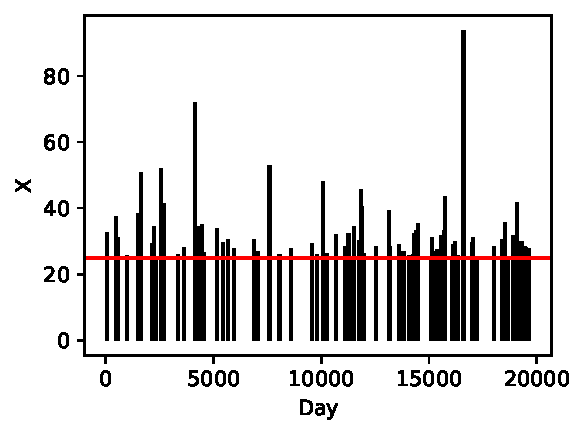
\includegraphics[width=0.32\linewidth]{plots/ppp-data.pdf}
	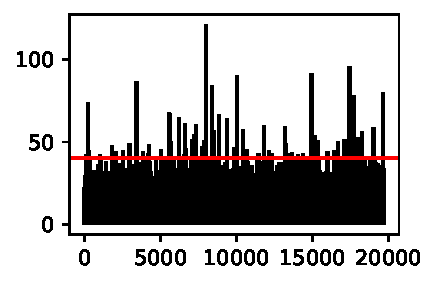
\includegraphics[width=0.32\linewidth]{plots/pd-data.pdf}
	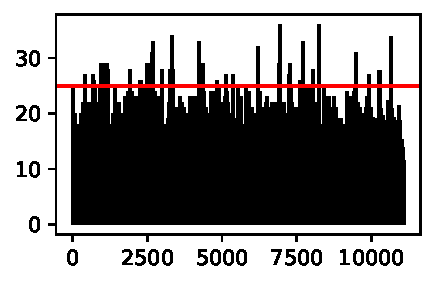
\includegraphics[width=0.32\linewidth]{plots/ws-data.pdf}
	\caption{PPP (left), PD (middle), and WD (right) datasets, with
		chosen thresholds in red}
	\label{fig:data}
\end{figure}
%

%
The analyses are coded in Python, using the libraries and packages
NumPy~(\cite{numpy}), Matplotlib~(\cite{matplotlib}),
SciPy~(\cite{scipy}), and OpenTURNS~(\cite{OpenTURNS}).
The code is available at \url{https://github.com/tzhg/extreme-bayes}.
Details of the Metropolis algorithm implementations
are tabulated in Appendix~\ref{section:mcmc-tables}.
%
\subsection{PPP: Poisson point process data}
%

%
According to the model described in \S~\ref{section:model},
the exceedances of the threshold $u$ approximately
follow a non-homogeneous Poisson point process with intensity function
%
\begin{align*}
	\lambda(x) = \frac{1}{\sigma}
		\left\{1 + \xi \left(\frac{x - \mu}{\sigma}\right)\right\}_+
		^ {-\frac{\xi + 1}{\xi}} \,.
\end{align*}
%
We simulated data for which this approximation is exact,
with known parameters.
We set $M = 54$ and $n_u = 86$
to match the study in \cite{coles1996}.
We choose parameters $\theta = (25, 5, 0.2)$,
and calculated the threshold $u$ using the equation
%
\begin{align*}
	M \Lambda[u, \infty) = n_u \\
	\iff u = \mu + \sigma \frac{\left(\frac{n_u}{M}\right)
		^ {-\xi} - 1}{\xi} \,,
\end{align*}
%
with $\Lambda$ defined in \eqref{eq:Lambda}.
This resulted in a threshold of $u = 22.778$.
The intensity function is equal to the PDF
of a Generalised Pareto distribution,
except with support $\{x \colon x > u\}$.
This means that we can simulate from the intensity
by simulating from a Generalised Pareto distribution
with parameters $(u, \sigma, \xi)$.
We simulated $86$ observations, and distributed them uniformly
over the total time period of $365 M$ observations,
setting the remaining points to $0$.
%

%
We constructed the priors
with the knowledge of the true quantiles and quantile differences.
Fixing $p = (0.1, 0.01, 0.001)$, then
%
\begin{align*}
	\tilde{q}^*_1 = 39.211 \,, \quad \tilde{q}^*_2 = 23.523 \,,
		\quad \tilde{q}^*_3 = 36.783
\end{align*}
%
are the true quantile differences.
To construct $\pi^{\text{G3}}_q$, we chose
%
\begin{align*}
	\tilde{q}_i \sim \Gamma\left(\frac{(\tilde{q}^*_i) ^ 2}{v},
		\frac{\tilde{q}^*_i}{v}\right) \,, \quad i = 1, 2, 3 \\
	\implies \E(\tilde{q}_i) = \tilde{q}^*_i, \quad \Var(\tilde{q}_i) = v
\end{align*}
%
for $v=5$.
For $\pi^{\text{MEC}}$, the approximation of quantile marginals
by Gamma distributions is shown in Fig.~\ref{fig:ppp-MEC-approx}.
For $\pi^{\text{TN}}$, the target mean and variance were
\input{latex-bits/ppp-TN-target.txt},
while the mean and variance of the constructed
truncated normal distributions were
\input{latex-bits/ppp-TN-approx.txt}.
%
\begin{figure}
	\centering
	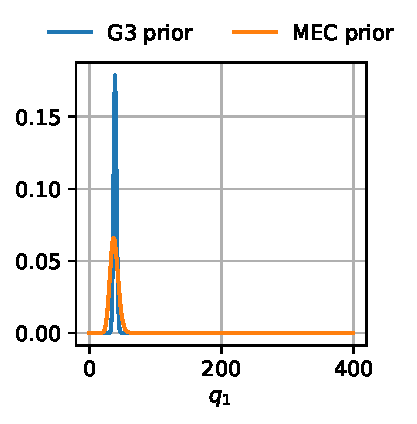
\includegraphics[width=0.32\linewidth]{plots/ppp-MEC-approx-0.pdf}
	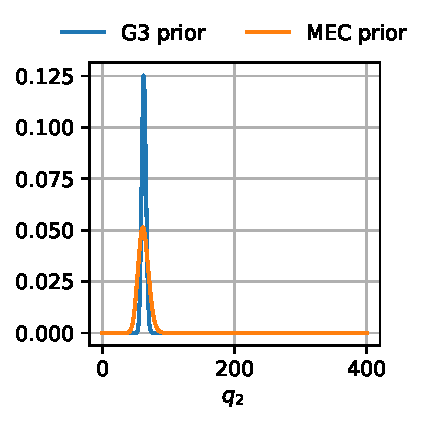
\includegraphics[width=0.32\linewidth]{plots/ppp-MEC-approx-1.pdf}
	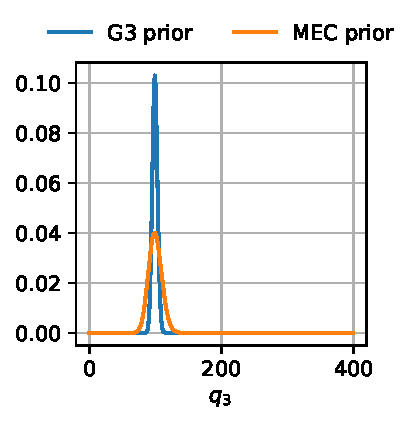
\includegraphics[width=0.32\linewidth]{plots/ppp-MEC-approx-2.pdf}
	\caption{Comparison of marginals of $\pi_{q}^{\text{G3}}$
		and $\pi_{q}^{\text{MEC}}$}
	\label{fig:ppp-MEC-approx}
\end{figure}
%

%
The univariate and bivariate marginals of
$\theta$ and $q_1, q_2, q_3$ for the different priors are illustrated
in Table~\ref{table:ppp-theta-0-marg}, Table~\ref{table:ppp-theta-1-marg},
Table~\ref{table:ppp-q-0-marg} and Table~\ref{table:ppp-q-1-marg}.
We plotted the mean return level compared to the analytic true return level
in Fig.~\ref{table:ppp-post-return-level}.
The dashed line was obtained by simulating $270,\!000$ years of data
and calculating the empirical quantiles.
%
\allmarginals{ppp}{Poisson process simulation study}
\allreturnlevels{ppp}{Poisson process simulation study}
%
\FloatBarrier
\subsection{PD: Pseudo-data}
%

%
In order to compare our results to \cite{coles1996},
we generated data, denoted $\mathbf{x}^{\text{PD}}$,
from $\operatorname{GEV}(17, 1.8, 0.28)$ to resemble their data, such that:
%
\begin{align*}
	\centering
	\renewcommand{\arraystretch}{1.2}
	\begin{tabular}{@{}ccc@{}}
		\toprule[0.1em]
		&$\mathbf{x}^{\text{PD}}$ &\cite{coles1996}\\
		\midrule[0.1em]
		$M$ &$54$ &$54$ \\
		$u$ &$40.109$ &$40$ \\
		$n_u$ &$86$ &$86$ \\
		\bottomrule[0.1em]
	\end{tabular}
\end{align*}
%

%
We used the same prior $\pi^{\text{G3}}_{\tilde{q}}$
for independent quantile differences as specified by \cite{coles1996}, given by
%
\begin{align*}
	p &= (0.1, 0.01, 0.001) \,,\\
	\tilde{q}_1 &\sim \Gamma(38.9, 0.67) \,,\\
	\tilde{q}_2 &\sim \Gamma(7.1, 0.16) \,,\\
	\tilde{q}_3 &\sim \Gamma(47, 0.39) \,.
\end{align*}
%
For $\pi^{\text{MEC}}$, the approximation of quantile marginals
by Gamma distributions is shown in Fig.~\ref{fig:pd-MEC-approx}.
For $\pi^{\text{TN}}$, the target mean and variance were
\input{latex-bits/pd-TN-target.txt},
while the mean and variance of the constructed
truncated normal distributions were
\input{latex-bits/pd-TN-approx.txt}.
%
\begin{figure}
	\centering
	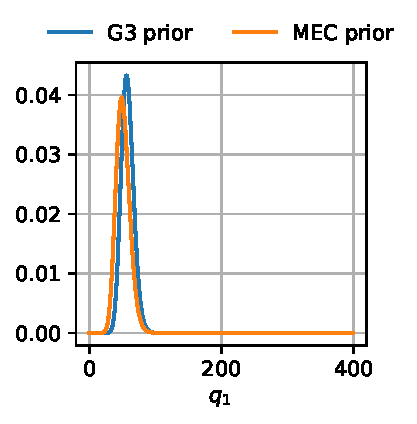
\includegraphics[width=0.32\linewidth]{plots/pd-MEC-approx-0.pdf}
	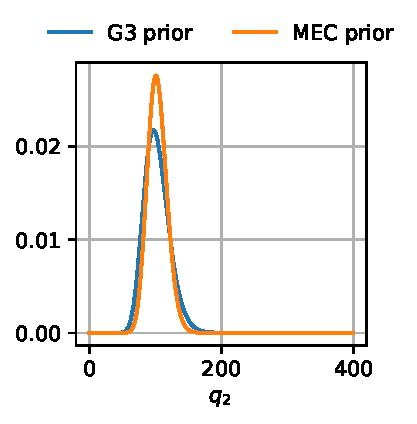
\includegraphics[width=0.32\linewidth]{plots/pd-MEC-approx-1.pdf}
	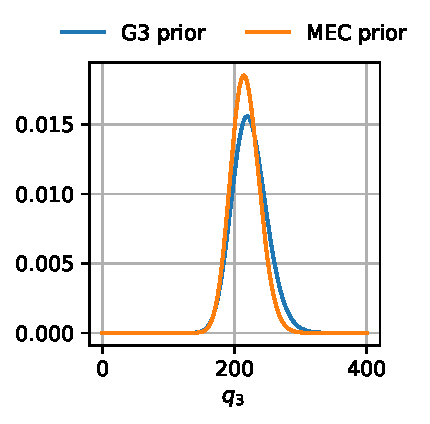
\includegraphics[width=0.32\linewidth]{plots/pd-MEC-approx-2.pdf}
	\caption{Comparison of marginals of $\pi_{q}^{\text{G3}}$
		and $\pi_{q}^{\text{MEC}}$}
	\label{fig:pd-MEC-approx}
\end{figure}
%

%
The univariate and bivariate marginals of
$\theta$ and $q_1, q_2, q_3$ for the different priors are illustrated
in Table~\ref{table:pd-theta-0-marg}, Table~\ref{table:pd-theta-1-marg},
Table~\ref{table:pd-q-0-marg} and Table~\ref{table:pd-q-1-marg}.
In Table~\ref{table:pd-validation},
we compare the statistics of the quantile differences
specified by the expert, to the statistics estimated
using the MCMC samples of $(\mu, \sigma, \xi)$ for each of the priors.
In Fig.~\ref{table:pd-post-return-level},
the mean return level is plotted with 95\% credibility intervals
and empirical quantiles. 
The dashed black line was obtained by simulating $270,\!000$ years of data
and calculating the empirical quantiles.
We know that the annual maximum has CDF $F^{365}$,
where $F$ is the CDF of $\operatorname{GEV}(17, 1.8, 0.28)$,
and the solid black line shows
the quantiles calculated analytically from this CDF.
%

%
In Fig.~\ref{fig:pd-vt}, we varied the threshold,
and plotted the number of exceedances against the return level
for return periods $10^2$, $10^3$, and $10^4$,
all estimated using the prior
$\pi_{\theta \mid \mathbf{x}^{\text{PD}}}^{\text{G3}}$.
%
\begin{table*}
	\centering
	\renewcommand{\arraystretch}{1.2}
	\begin{tabular}{@{}ccccc@{}}
		\toprule[0.1em]
		&$\tilde{q}_1$ &$\tilde{q}_2$ &$\tilde{q}_3$ \\
		\midrule[0.1em]
		Expert &$(57.563, 70.263)$ &$(42.310, 66.805)$ &$(119.09, 142.836)$ \\
		\input{latex-bits/pd-prior-quantiles.txt}
		\bottomrule[0.1em]
	\end{tabular}
	\caption{Pairs of $(\text{median}, 0.9\text{-quantile})$ of quantile differences 
		for pseudo-data simulation study}
	\label{table:pd-validation}
\end{table*}
%
\allmarginals{pd}{pseudo-data simulation study}
%
\begin{figure}
	\centering
	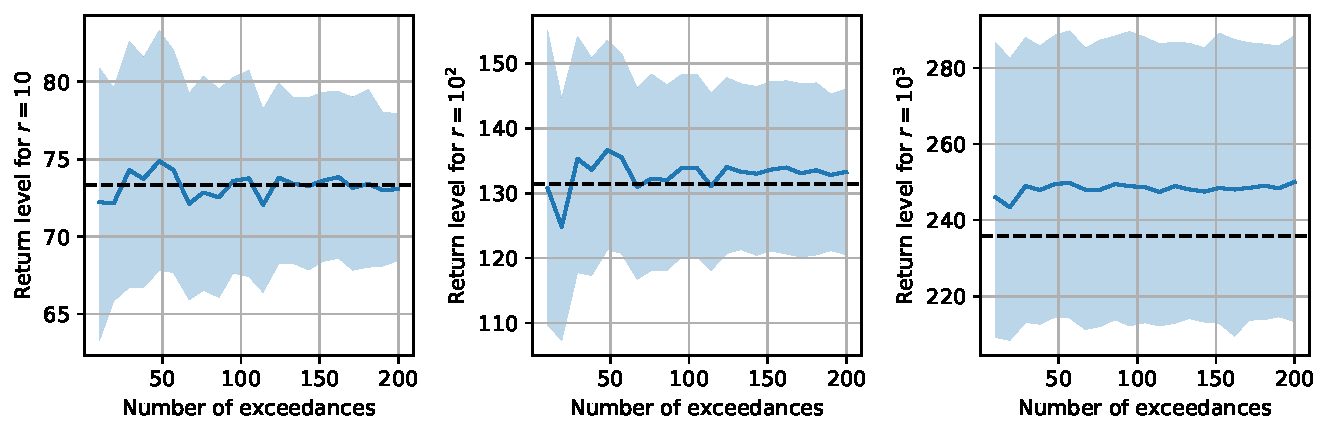
\includegraphics[width=0.9\linewidth]{plots/pd-vt.pdf}
	\caption{Mean return levels {\color{blue} \textbf{(blue)}}
		with 95\% credibility intervals
		estimated using $\pi_{\theta \mid \mathbf{x}^{\text{PD}}}^{\text{G3}}$
		for various thresholds,
		with simulated return levels {\color{black} \textbf{(black dashed)}}}
	\label{fig:pd-vt}
\end{figure}
%
\allreturnlevels{pd}{pseudo-data process simulation study}
%
\FloatBarrier
\subsection{WS: Daily average wind speed}
%

%
This dataset consists of observations of average wind speed
at Tours, France over a period of $30.34$ years, from 1981 to 2011.
We chose a threshold of $u = 25$ with $76$ exceedances.
%

%
In order to construct the priors,
We first fitted a GEV distribution on the annual maxima of the data.
The Q-Q plot is shown in Fig.~\ref{fig:ws-qq}.
%
\begin{figure}
	\centering
	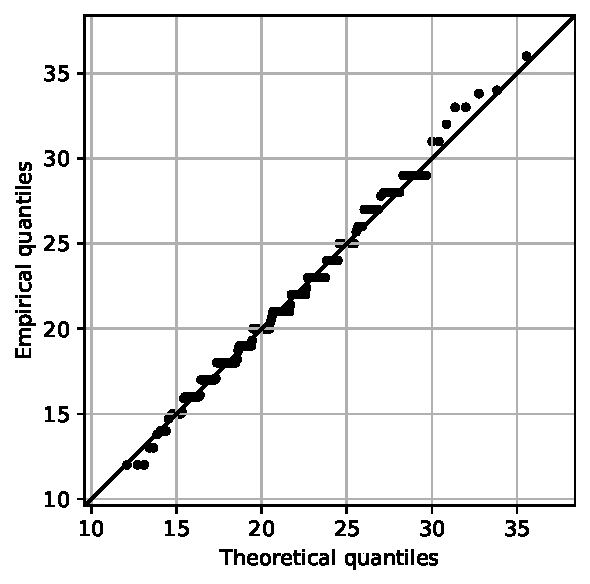
\includegraphics[width=0.7\linewidth]{plots/ws-qq.pdf}
	\caption{Q-Q plot of GEV distribution fit for wind speed data}
	\label{fig:ws-qq}
\end{figure}
%
The estimated corresponding quantiles differences estimates
were then obtained, and Gamma distributions centred on these estimates
were constructed with variance $5$.
For $\pi^{\text{MEC}}$, the approximation of quantile marginals
by Gamma distributions is shown in Fig.~\ref{fig:ws-MEC-approx}.
For $\pi^{\text{TN}}$, the target mean and variance were
\input{latex-bits/ws-TN-target.txt},
while the mean and variance of the constructed
truncated normal distributions were
\input{latex-bits/ws-TN-approx.txt}.
%
\begin{figure}
	\centering
	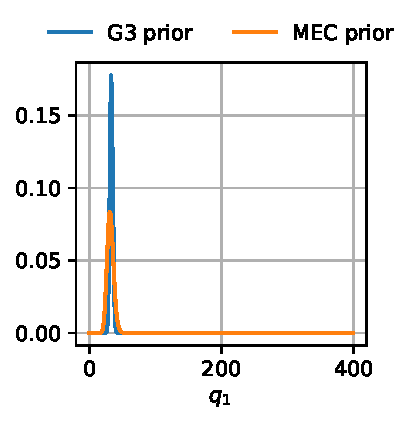
\includegraphics[width=0.32\linewidth]{plots/ws-MEC-approx-0.pdf}
	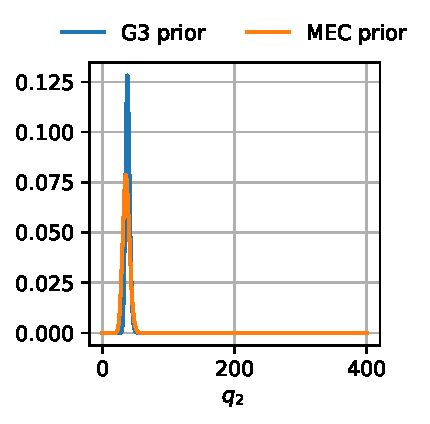
\includegraphics[width=0.32\linewidth]{plots/ws-MEC-approx-1.pdf}
	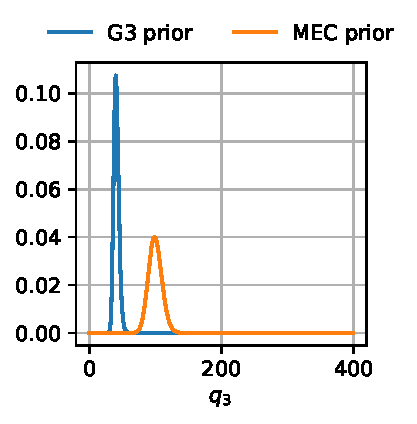
\includegraphics[width=0.32\linewidth]{plots/ws-MEC-approx-2.pdf}
	\caption{Comparison of marginals of $\pi_{q}^{\text{G3}}$
		and $\pi_{q}^{\text{MEC}}$}
	\label{fig:ws-MEC-approx}
\end{figure}
%

%
The univariate and bivariate marginals of
$\theta$ and $q_1, q_2, q_3$ for the different priors are illustrated
in Table~\ref{table:ws-theta-0-marg}, Table~\ref{table:ws-theta-1-marg},
Table~\ref{table:ws-q-0-marg} and Table~\ref{table:ws-q-1-marg}.
We plotted the mean return level in Fig.~\ref{table:ws-post-return-level}.
%
\allmarginals{ws}{wind speed data}
\allreturnlevels{ws}{wind speed data}
%
\FloatBarrier
\appendix
%
\section{Maximum entropy distributions}
\label{section:max_entropy_proofs}
%

%
In order to find the distribution which maximises
the entropy under certain constraints,
we will use Lagrange multipliers and calculus of variations.
Let $p$ be a probability density with support $(0, +\infty)$.
That is,
%
\begin{align*}
	\int_0^{+\infty} p(x) \, \dd x = 1 \,, \\
	p(x) > 0 \quad \forall x \in (0, +\infty) \,.
\end{align*}
We define entropy as
%
\begin{align*}
	{\cal E}(p) = -\int_0^{+\infty} p(x) \log(p(x)) \, \dd x \,,
\end{align*}
%
where we take the  natural logarithm instead of the base 2 logarithm,
as this simplifies the calculation without changing the results.
We define $n$ constraints in the form
\begin{align*}
	\int_0^{+\infty} p(x) f_i(x) \, \dd x - c_i \,, \quad i = 1, \dots, n \,.
\end{align*}
%
for measurable functions $f_i$.
Therefore, we obtain the objective function
%
\begin{align*}
	L(p, \lambda) &= -\int_0^{+\infty} p(x) \log(p(x)) \, \dd x
		+ \lambda_0 \left(\int_0^{+\infty} p(x) \, \dd x - 1\right) \\
	&\ \phantom{=} + \sum_{i=1}^n \lambda_i
		\left(\int_0^{+\infty} p(x) f_i(x) \, \dd x - c_i\right) \,.
\end{align*}
%
It has partial derivatives
\begin{align*}
	\frac{\partial L}{\partial p}(p)
		&= -\log (p(x)) - 1 + \lambda_0 + \sum_{i = 1}^n \lambda_i f_i(x) \\
	\frac{\partial ^ 2 L}{\partial p ^ 2}(p)
		&= -\frac{1}{p(x)} \,,
\end{align*}
%
and setting $\frac{\partial L}{\partial p} = 0$,
we get that for all $x \in (0, +\infty)$,
%
\begin{align}
	\frac{\partial L}{\partial p} = 0 &\iff p(x)
		= \exp\left(1 - \lambda_0 + \sum_{i = 1}^n \lambda_i f_i(x)\right)
		\,, \nonumber\\
	&\implies p(x) \propto \exp\left(\sum_{i = 1}^n \lambda_i f_i(x)\right) \,. 
	\label{eq:p-prop}
\end{align}
%
\subsection*{Fixed quantiles}
%
Given $n$ probabilities $p_i$, and their corresponding $p_i$-quantiles $q_i$,
the constraints have the form
\begin{align*}
	f_i(x) = \mathbbm{1}_{(0, q_i)}(x) \,, &\quad c_i = p_i \\
\end{align*}
%
and therefore from \eqref{eq:p-prop},
%
\begin{align*}
	p(x) \propto \exp\left(\sum_{i = 1}^n \lambda_i
		\mathbbm{1}_{(0, q_i)}(x) \right)
		&= \sum_{i = 1}^n \exp\left(\lambda_i \right) 
		\mathbbm{1}_{(0, q_i)}(x) \,.
\end{align*}
%
This implies that the maximum entropy distribution is proportional to a
piecewise uniform distribution on $(0, +\infty)$.
However, such a distribution doesn't exist.
%
\subsection*{Fixed mean}
%
Given mean $\mu$, the constraint has the form
\begin{align*}
	f_1(x) = x \,, \quad c_1 = \mu \,,
\end{align*}
%
and therefore from \eqref{eq:p-prop},
%
\begin{align*}
	p(x) \propto \exp\left(\lambda_1 x \right) \,.
\end{align*}
%
This implies that the maximum entropy distribution
is an exponential distribution.
%
\subsection*{Fixed mean and variance}
%
Given mean $\mu$ and variance $\sigma ^ 2$, the constraints have the form
\begin{align*}
	f_1(x) = x \,, &\quad c_1 = \mu \\
	f_2(x) = x ^ 2 \,, &\quad c_2 = \sigma ^ 2 + \mu ^ 2 \,,
\end{align*}
%
and therefore from \eqref{eq:p-prop},
%
\begin{align*}
	p(x) \propto \exp\left(\lambda_1 x + \lambda_2 x ^ 2\right) \,.
\end{align*}
%
This implies that the maximum entropy distribution is a normal distribution,
truncated to $(0, +\infty)$.
%
\section{Obtaining truncated normal parameters from mean and variance}
\label{section:tn-invert}
%

%
Suppose that we are given the mean $\mu^*$ and variance $(\sigma^*) ^ 2$
of a random variable $X$ which follows a truncated normal distribution
with support parameters $a = 0$ and $b = +\infty$,
and we would like to determine the remaining parameters $\mu$ and $\sigma$.

%
This means that we need to invert the equations
%
\begin{align*}
	\E(X) &= \mu + \frac{\phi(\alpha)}{1 - \Phi(\alpha)} \sigma \\
	\Var(X) &= \sigma ^ 2 \left(1 + \frac{\alpha \phi(\alpha)}{1 - \Phi(\alpha)}
		- \left(\frac{\phi(\alpha)}{1 - \Phi(\alpha)}\right) ^ 2\right) \,,
\end{align*}
%
where $\phi$ and $\Phi$ are the PDF and CDF of the
standard normal distribution respectively and
%
\begin{align}
	\alpha \coloneqq -\frac{\mu}{\sigma} \,.
	\label{tn-alpha}
\end{align}
%
Setting
%
\begin{align*}
	H(x) \coloneqq \frac{\phi(x)}{1 - \Phi(x)} \,,
\end{align*}
%
which is the hazard function of the standard normal distribution, we can
simplify the equations to
%
\begin{align}
	\E(X) &= \mu + H(\alpha)\sigma \label{tn-mean} \\
	\Var(X) &= \sigma ^ 2 \left(1 + \alpha H(\alpha) - (H(\alpha)) ^ 2 \right)
		\label{tn-var} \,.
\end{align}
%
Therefore,
%
\begin{align*}
	\left(\frac{\sigma^*}{\mu^*}\right)^2 &=
		\frac{\sigma ^ 2 \left(1 + \alpha H(\alpha) - (H(\alpha)) ^ 2 \right)}{%
		\left(\mu + H(\alpha) \sigma\right) ^ 2} \\
	&= \frac{1 + \alpha H(\alpha) - (H(\alpha)) ^ 2}
		{\left(H(\alpha) - \alpha\right) ^ 2} \eqqcolon f(\alpha) \,, \\
\end{align*}
%
and once we have $\alpha$, from \refeq{tn-mean} we have
%
\begin{align*}
	\frac{\mu^*}{\sigma} = H(\alpha) - \alpha
		\implies \sigma = \frac{\mu^*}{H(\alpha) - \alpha}
\end{align*}
%
and from \refeq{tn-alpha},
%
\begin{align*}
	\alpha = -\frac{\mu}{\sigma} \implies \sigma =  -\alpha \mu \,.
\end{align*}
%
It remains to solve $f(\alpha) = \left(\frac{\sigma^*}{\mu^*}\right) ^ 2$.
This can be done numerically using Newton's method with the derivative of $f$.
Since
%
\begin{align*}
	\phi'(x) = -x \phi(x) \,,
\end{align*}
%
the derivative of $H$ is
%
\begin{align*}
	H'(x) &= \frac{(1 - \Phi(x)) x (-\phi(x))
		- \phi(x)(- \phi(x))}{(1 - \Phi(x))^2} \\
	&= \phi(x) \frac{-(1 - \Phi(x)) x + \phi(x)}
		{(1 - \Phi(x))^2} \\
	&= H(x) \frac{-(1 - \Phi(x)) x + \phi(x)}
		{1 - \Phi(x)} \\
	&= H(x) \left(\frac{-(1 - \Phi(x)) x}
		{1 - \Phi(x)} + H(x) \right) \\
	&= H(x) \left(H(x) - x \right) \,.
\end{align*}
%
Therefore the derivative of $f$ is
%
\begin{align*}
	f'(x) &= \left(\left(H(x) - x\right) ^ 2
		\left(H(x) + x H(x) \left(H(x) - x \right)
		- 2 (H(x)) ^ 2 \left(H(x) - x \right)\right)\right. \\
	&\ \phantom{=} \left. - \left(1 + x H(x) - (H(x)) ^ 2\right)
		2 \left(H(x) - x\right) \left(H(x) \left(H(x) - x \right) - 1\right)\right)
		\left(H(x) - x\right) ^ {-4} \\
	&= \frac{(2 + H(x) (H(x) - x) (-3 + (H(x) - x) x))}{(H(x) - x) ^ 3} \,.
\end{align*}
%
%
\section{Maximum entropy copula condition (C2)}
\label{section:C2}
%

%
The construction of the maximum entropy distribution in
\S~\ref{section:prior-mec} requires the following condition on the marginals:
for a sequence of distributions $(F_i)_{1 \geq i \geq d}$,
%
\begin{align*}
	\textit{(C2)} \coloneqq \forall 1 \leq i \leq d - 1
		\ \forall x \in \{x \colon 1 > F_i(x), F_{i + 1}(x) > 0\}
		\ (F_i(x) > F_{i + 1}(x))\,.
\end{align*}
%
We will investigate this condition for Weibull and Gamma distributed marginals.
%
\subsection*{Weibull distribution}
%
Let $1 \leq i \leq d - 1$. We have that
%
\begin{align*}
	1 > F_i(x), F_{i + 1}(x) > 0 \iff x > 0 \,.
\end{align*}
%
The CDF when $x > 0$ is
%
\begin{align*}
	F_i(x) = 1 - \exp\left(-\left(\frac{x}{\lambda_i}\right) ^ {k_i}\right) \,,
\end{align*}
%
with $k_i$, $\lambda_i > 0$. Let $ x> 0$. Then
%
\begin{align*}
	\textit{(C2)} & \iff 1 - \exp\left(-\left(\frac{x}{\lambda_i}\right)
		^ {k_i}\right) > 1- \exp\left(-\left(\frac{x}{\lambda_{i + 1}}\right)
		^ {k_{i + 1}}\right)\\
	&\iff \left(\frac{x}{\lambda_i}\right) ^ {k_i} >
		\left(\frac{x}{\lambda_{i + 1}}\right) ^ {k_{i + 1}} \,.
\end{align*}
%
If $k_i = k_{i + 1} = k$,
%
\begin{align*}
	\left(\frac{x}{\lambda_i}\right) ^ k
		> \left(\frac{x}{\lambda_{i + 1}}\right) ^ k&
		\iff \frac{x}{\lambda_i} > \frac{x}{\lambda_{i + 1}}\\
	&\iff \frac{1}{\lambda_i} > \frac{1}{\lambda_{i + 1}}\\
	&\iff \lambda_i < \lambda_{i + 1} \,.
\end{align*}
%
If $k_i \neq k_{i + 1}$,
%
\begin{align*}
	F_i(x) =F_{i + 1}(x)
		&\iff \left(\frac{x}{\lambda_i}\right) ^ {k_i}
		= \left(\frac{x}{\lambda_{i + 1}}\right) ^ {k_{i + 1}}\\
	&\iff \exp\left(k_i (\log x - \log\lambda_i)\right)
		=\exp\left({k_{i + 1}}(\log x - \log\lambda_{i + 1})\right)\\
	&\iff k_i (\log x - \log\lambda_i)
		= {k_{i + 1}} (\log x - \log\lambda_{i + 1})\\
	&\iff k_i \log x - k_i \log\lambda_i 
		= {k_{i + 1}} \log x - {k_{i + 1}} \log\lambda_{i + 1}\\
	&\iff k_i \log x - {k_{i + 1}} \log x
		=k_i \log\lambda_i - {k_{i + 1}} \log\lambda_{i + 1}\\
	&\iff (k_i - {k_{i + 1}}) \log x 
		= k_i \log\lambda_i - {k_{i + 1}} \log\lambda_{i + 1}\\
	&\iff \log x
		= \frac{k_i \log\lambda_i - {k_{i + 1}}
		\log\lambda_{i + 1}}{k_i - {k_{i + 1}}}\\
	&\iff x
		= \exp\underbrace{\left(\frac{k_i \log\lambda_i - {k_{i + 1}}
		\log\lambda_{i + 1}}{k_i - {k_{i + 1}}}\right)}
		_{\eqqcolon h(k_i, \lambda_i, k_{i + 1}, \lambda_{i + 1})} \,.
\end{align*}
%
Therefore the two CDFs intersect, and so $\textit{(C2)}$ cannot be satisfied.
In conclusion,
%
\begin{align*}
	\textit{(C2)}
		&\iff (k_i = k_{i + 1}) \land (\lambda_i < \lambda_{i + 1})
		\quad \forall 1 \leq i \leq d - 1 \,.
\end{align*}
%

%
%In practice however, as
%$y \coloneqq h(k_i, \lambda_i, k_{i+1}, \lambda_{i+1}) \to \pm \infty$,
%the intersection will tend to the bounds of the set
%$\{x \colon 1 > F_i(x), F_{i + 1}(x) > 0\}$ and so $\textit{(C2)}$
%will be asymptotically satisfied. When does this happen?
%Consider a reparametrisation
%%
%\begin{align*}
%	(k_i, \lambda_i, k_{i + 1}, \lambda_{i + 1}) \mapsto
%		(k_i, \lambda_i, k_i - {k_{i + 1}}, \lambda_{i + 1}) \,,
%\end{align*}
%%
%which implies that
%%
%\begin{align*}
%	h(k_i, \lambda_i, z_{i}, \lambda_{i+1})
%		=\frac{k_i \log\lambda_i + {(z_{i} - k_{i})}
%		\log\lambda_{i + 1}}{z_{i}} \,,
%		\quad z_{i} < k_i,\ z_{i} \neq 0 \,.
%\end{align*}
%%
%Then
%%
%\begin{itemize}
%	\item As $z_i \to 0$, $y \to +\infty$,
%	\item As $k_i \to +\infty$, $y \to \pm\infty$, with sign depending
%		on the sign of $\log(\frac{\lambda_i}{\lambda_{i + 1}})$,
%	\item As $\lambda_i \to +\infty$ or $\lambda_{i + 1} \to 0$,
%		$y \to +\infty$,
%	\item As $\lambda_i \to 0$ or  $\lambda_{i + 1}\to +\infty$,
%		$y \to -\infty$.
%\end{itemize}
%%
\subsection*{Gamma distribution}
%

%
Let $1 \leq i \leq d - 1$. We have that
%
\begin{align*}
	1 > F_i(x), F_{i+1}(x) > 0 \iff x > 0 \,.
\end{align*}
%
Suppose that we have two such distributions,
%
\begin{align*}
	F_1(x) = \frac{\beta^{\alpha_1}_1}{\Gamma(\alpha_1)} x ^ {\alpha_1}
	\exp(\beta_1 x) \quad \text{and} \quad
	F_2(x) = \frac{\beta^{\alpha_2}_2}{\Gamma(\alpha_2)} x ^ {\alpha_2}
	\exp(\beta_2 x) \,,
\end{align*}
%
with $\alpha_i, \beta_i > 0$ the shape and rate parameters.
Denote their respective PDFs by $f_1$ and $f_2$.
Let $x > 0$, and define
%
\begin{align*}
	\phi(x) = F_2(x) - F_1(x) \,,
\end{align*}
%
so that if $(i, i + 1) = (1, 2)$,
%
\begin{align*}
	\textit{(C2)} \iff \phi(x) < 0 \,,
\end{align*}
%
and if $(i, i + 1) = (2, 1)$,
%
\begin{align*}
	\textit{(C2)} \iff \phi(x) > 0 \,.
\end{align*}
%
We have that
%
\begin{align*}
	\phi'(x) &= f_2(x) - f_1(x)\\
	&= f_1(x) \left(\frac{f_2(x)}{f_1(x)} - 1\right)\\
	&= f_1(x) \left(\frac{\Gamma(\alpha_1)\beta ^ {\alpha_2}_2}
		{\Gamma(\alpha_2)\beta ^ {\alpha_1}_1} x^{\alpha_2 - \alpha_1}
		\exp((\beta_1 - \beta_2) x) - 1\right) \,.
\end{align*}
%
Let
%
\begin{align*}
	C \coloneqq \frac{\Gamma(\alpha_1) \beta ^ {\alpha_2}_2}
		{\Gamma(\alpha_2) \beta ^ {\alpha_1}_1} > 0
\end{align*}
%
and
%
\begin{align*}
	f(x) \coloneqq C x ^ {\alpha_2 - \alpha_1}
		\exp((\beta_1 - \beta_2) x) - 1 \,.
\end{align*}
%
Then
%
\begin{align*}
	f'(x) &= C\left[(\alpha_2 - \alpha_1) x ^ {\alpha_2 - \alpha_1 - 1}
		\exp((\beta_1 - \beta_2) x) + x ^ {\alpha_2 - \alpha_1}
		\exp((\beta_1 - \beta_2) x)(\beta_1 - \beta_2) \right]\\
	&=\underbrace{C x ^ {\alpha_2 - \alpha_1 - 1} \exp((\beta_1 - \beta_2) x)}
		_{ > 0} \left[(\alpha_2 - \alpha_1) + x (\beta_1 - \beta_2)\right]
\end{align*}
%
\subsubsection*{\underline{Case 1:
	$(\alpha_1 \leq \alpha_2 \land \beta_1 \geq \beta_2)
	\land \neg (\alpha_1 = \alpha_2 \land \beta_1 = \beta_2)$}}
%

%
We have that $\alpha_2 - \alpha_1 \geq 0$ and
$\beta_1 - \beta_2 \geq 0$, and therefore
%
\begin{align*}
	(\alpha_2 - \alpha_1) + x(\beta_1 - \beta_2) &> 0\\
	\implies f'(x) & > 0 \,.
\end{align*}
%
This implies that $f$ is strictly increasing on $\R^+$.
%
\begin{enumerate}
	\item If $\alpha_1 < \alpha_2$, we have that
		\begin{align*}
			\lim_{x \to 0^+} f(x) = -1 \quad \text{and} \quad
				\lim_{x \to +\infty} f(x) = +\infty\,.
		\end{align*}
	\item If $\alpha_1 = \alpha_2 = \alpha$ and $\beta_1 > \beta_2$,
		we have that
		\begin{align*}
			\lim_{x \to 0^+} f(x)
				= \left(\frac{\beta_2}{\beta_1}\right) ^ \alpha - 1 < 0 \quad
				\text{and} \quad \lim_{x \to +\infty} f(x) = +\infty \,.
		\end{align*}
\end{enumerate}
%
Therefore in both cases, there exists a unique $z_0 > 0$
such that $f(z_0) = 0$. This implies that
%
\begin{align*}
	\begin{cases}
		\phi'(x) < 0 &\text{if} \quad x < z_0 \,,\\
		\phi'(x) = 0 &\text{if} \quad x = z_0 \,,\\
		\phi'(x) > 0 &\text{if} \quad x > z_0 \,.
	\end{cases}
\end{align*}
%
In order to proceed we will need the following Lemma.
%
\begin{lemma}
	\begin{enumerate}
		\item Let $f \colon (a, b] \to \R$ be continuous on $(a, b]$
			and differentiable on $(a, b)$, with 
			$a \in \R \cup \{+\infty\}, b \in \R$. If for all $x \in (a, b)$,
			\ $f'(x) > 0$ (resp. $<$) and $\lim_{x \to a^+} f(x) = L \in \R$,
			then for all $z \in (a, b]$, $f(z) > L$ (resp. $<$).
		\item Let $f \colon [a, b) \to \R$ be continuous on $[a, b)$
			and differentiable on $(a, b)$, with
			$a \in \R, b \in \R \cup \{+\infty\}$. If for all $x\in(a, b)$,
			\ $f'(x) > 0$ (resp. $<$) and $\lim_{x \to b^-} f(x) = L \in \R$,
			then for all $z \in [a, b)$, $f(z) < L$ (resp. $>$).
	\end{enumerate}
	\label{lemma:limit}
\end{lemma}
%
\begin{proof}
	We will prove the first case, for $f'(x) > 0$,
	as both cases are symmetrical. Suppose that $z \in (a, b)$.
	We need to show that $f(z),f(b) > L$. Let $y \in (a, z)$.
	As $f'$ is strictly positive on $(a, b)$, $f$ is strictly increasing
	(by the mean value theorem), and so $f(z) - f(y) = c > 0$.
	Therefore $f(z) > f(y) + \frac{c}{2}$.
	Then $f(z) = \lim_{y \to a^+} f(z) \geq \lim_{y \to a^+} f(y)
	+ \frac{c}{2} = L + \frac{c}{2} > L$.
	Furthermore, $f(b) = \lim_{z \to b^-} f(z) \geq \lim_{x \to b^-} 
	(L + \frac{c}{2}) = L + \frac{c}{2} > L$.
\end{proof}
%

%
By Lemma~\ref{lemma:limit}, for all $z \in (0, z_0]$,
$\phi(z) < \lim_{x\to 0^+}\phi(x)=0$, and for all $z \in[z_0, +\infty)$,
$\phi(z) < \lim_{x \to +\infty} \phi(x) = 0$.
Therefore for all $x > 0$, $\phi(x) < 0$, and so if $(i, i + 1)=(1, 2)$,
(C2) is satisfied, and if $(i, i + 1) = (2, 1)$, (C2) is violated.
%
\subsubsection*{\underline{Case 2: $\alpha_1 < \alpha_2, \  \beta_1 < \beta_2$}}
%

%
Since
%
\begin{align*}
	\lim_{x \to 0^+} f(x) = -1 \,,
\end{align*}
%
there exists a $\delta > 0$ such that for all $z \in (0, \delta]$,
$f(z) = \phi'(z) < 0$, and so by Lemma~\ref{lemma:limit},
$\phi(z) < \lim_{x \to 0^+} \phi(x) = 0$. Since
%
\begin{align*}
	\lim_{x \to +\infty} f(x) = -1 \,,
\end{align*}
%
there exists a $\delta' > 0$ such that for all $z \in [\delta', +\infty)$,
$f(z) = \phi'(z) < 0$, and so by Lemma~\ref{lemma:limit},
$\phi(z) > \lim_{x \to 0^+} \phi(x) = 0$.
Therefore $\phi$ is neither strictly positive nor strictly negative,
and so if either $(i, i + 1) = (1, 2)$ or
$(i, i + 1) = (2, 1)$, (C2) is violated.
%

%
In conclusion, we have shown that
%
\begin{align*}
	\textit{(C2)} \iff (\alpha_i \leq \alpha_{i + 1} \land \beta_{i}
	\geq \beta_{i + 1}) \land \neg(\alpha_i = \alpha_{i+1} \land \beta_i
	= \beta_{i + 1}) \quad \forall 1 \leq i\leq d - 1 \,.
\end{align*}
%
%Like in the Weibull case, the condition can be asymptotically satisfied.
%For instance, if the means $\frac{\alpha}{\beta}$ are sufficiently separated,
%and the variances $\frac{\alpha}{\beta ^ 2}$ are small,
%there will be less significant overlap between the CDFs.
%
\section{Metropolis-Hastings algorithm implementation details}
\label{section:mcmc-tables}
%

%
In Tables~\ref{table:pd-1}-\ref{table:ws-2}, we show details on our
implementations of the Metropolis-Hastings algorithm, including
the proposal distributions, initialisation, sample size, traceplots,
histograms, and acceptance rates.
%
\metroall{ppp}{PPP}{Poisson process simulation study}
\metroall{pd}{PD}{pseudo-data simulation study}
\metroall{ws}{WS}{wind speed data}
%
\FloatBarrier
%
\subsection{SS: Spike-and-slab prior distribution for \boldmath$\xi$}
\label{section:prior-ss}
%

%
This is a prior with a non-zero probability mass (spike) at $\xi = 0$,
and a flat slab elsewhere.
%

%
We use the method proposed by \cite{kuo1998}.
We introduce an indicator random variable $\gamma$ such that
$\gamma = 0$ when $\xi$ is ``in'' the spike
and $\gamma = 1$ when $\xi$ is ``in'' the slab.
The probability that $\xi$ is nonzero can then be calculated
as the mean of $\gamma$.
We also need a random variable $\beta$ such that $\xi = \beta \gamma$,
which determines the distribution of $\xi$ in the slab.
Our model now has parameters $\eta \coloneqq (\mu, \sigma, \beta, \gamma)$,
and we suppose that $\gamma$ does not depend on the other parameters.
%

%
If we have a prior $\pi_\theta$ for $(\mu, \sigma, \xi)$, then we can set
%
\begin{align*}
	\pi_{\mu, \sigma, \beta}^{\text{SS}} &\coloneqq \pi_\theta \\
	\pi_\gamma^{\text{SS}}(\gamma)
		&\coloneqq \alpha ^ \gamma (1 - \alpha) ^ {1 - \gamma} \\
	\implies \pi_{\eta}^{\text{SS}}(\eta)
		&= \pi_\theta(\mu, \sigma, \beta)
		\alpha ^ \gamma (1 - \alpha) ^ {1 - \gamma} \,,
\end{align*}
%
with $\alpha \in [0, 1]$. The posterior is then proportional to
%
\begin{align*}
	\pi_{\eta \mid \mathbf{x}}^{\text{SS}}(\eta \mid \mathbf{x}) &\propto
		L(\mu, \sigma, \beta \gamma \mid \mathbf{x})
		\pi_\theta(\mu, \sigma, \beta)
		\alpha ^ \gamma (1 - \alpha) ^ {1 - \gamma} \,.
\end{align*}
%

%
Since, up to the same constant of proportionality, we have
%
\begin{align*}
	\pi_{\gamma \mid \mu, \sigma, \beta, \mathbf{x}}^{\text{SS}}
		(0 \mid \mu, \sigma, \beta, \mathbf{x}) &\propto
		(1 - \alpha) L(\mu, \sigma, 0 \mid \mathbf{x})
\end{align*}
and
\begin{align*}
	\pi_{\gamma \mid \mu, \sigma, \beta, \mathbf{x}}^{\text{SS}}
		(1 \mid \mu, \sigma, \beta, \mathbf{x}) &\propto
		\alpha L(\mu, \sigma, \beta \mid \mathbf{x}) \,,
\end{align*}
%
the full conditional of $\gamma$ is a Bernoulli distribution
with probability of success
%
\begin{align*}
	\frac{\alpha L(\mu, \sigma, \beta \mid \mathbf{x})}
		{\alpha L(\mu, \sigma, \beta \mid \mathbf{x})
		+ (1 - \alpha) L(\mu, \sigma, 0 \mid \mathbf{x})} \,.
\end{align*}
%

%
We set $\pi_\theta = \pi_\theta^{\text{G3}}$,
and for an uninformative prior on $\gamma$, we set $\alpha = 0.5$.
%
\printbibliography
%
\end{document}